%% cls: https://raw.githubusercontent.com/HenryJi529/MorningstarPaper/main/morningstar.cls

\documentclass[twocolumn]{morningstar}
\title{基于深度强化学习的复杂网络节点影响力排序算法}
\entitle{Node Influence Ranking Algorithm in Complex Networks Based by Deep Reinforcement Learning}
\author{吉普}
\enauthor{Pu Ji}
\phone{19850052801}
\email{221307020006@hhu.edu.cn}
\location{南京}
\enlocation{Nanjing}
\organization{河海大学计算机与信息学院}
\enorganization{School of Computer and Information Science, Hohai University}

% \setcounter{section}{-1}

\begin{document}

\twocolumn[
    \thispagestyle{firstpage}
    \showcntitle
    \showauthor
    \showcnabstract{
        图数据的在各个领域的广泛运用和现实世界网络连接的复杂性,使得如何在已知网络拓扑的前提下,快速准确地评估复杂通信网络中的节点影响力成为当前的研究热点。
        本文提出了一种基于深度强化学习的节点影响力排序算法。
        这一算法从网络拆解的视角看待节点影响力,使用深度强化学习优化节点的拆除策略,进而获得节点的影响力排序。
        此外,本文所提出的算法还利用排序学习进行预训练来增强图神经网络的节点特征提取,并将节点嵌入向量应用于节点影响力的价值学习。
        本文所提出的算法在保持了接近朴素算法高准确度的同时,还实现了较低的时间复杂度,并且具有良好的泛化能力和实用性。
        未来的研究可以进一步探索和改进这种算法,以应对不断增长的网络复杂性和规模的挑战。
    }
    \showcnkeywords{
        节点影响力;复杂网络;强化学习;图神经网络;排序学习
    }
    \showentitle
    \showenauthor
    \showenabstract{
        The wide application of graph data in various fields and the complexity of real-world network connectivity make it a current research hotspot to quickly and accurately assess node influence in complex communication networks with known network topology.
        In this paper, we propose a node influence ranking algorithm based on deep reinforcement learning.
        This algorithm views node influence from the perspective of network dismantling and uses deep reinforcement learning to optimize the node dismantling strategy and thus obtain the influence ranking of nodes.
        In addition, the algorithm proposed in this paper utilizes Learning-To-Rank for pre-training to enhance node feature extraction in graph neural network and applies node embedding vectors to value-based reinforcement learning of node influence.
        The proposed algorithm achieves low time complexity while maintaining high accuracy close to the naive algorithm, and has good generalization ability and practicality.
        Future research can further explore and improve this algorithm to meet the challenges of growing network complexity and size.
    }
    \showenkeywords{
        Node Influence; Complex Network; Reinforcement Learning; Graph Nerual Network; Learning-To-Rank
    }
    ]

\section*{引言}\label{sec:Introduction}
现实世界中存在诸多相互关联、结构复杂的系统如互联网、交通系统、金融系统、社交关系、生态系统等,他们都可以被抽象为复杂网络。
网络科学的研究表明,现实世界中的网络并不都是随机网络,相反,更多的呈现出幂律分布的特性\cite{barabasi1999幂律分布}。
这一特性使得网络深受其中一小部分影响力大的节点的影响,这些节点的激活/断连将显着改善/降低某些网络功能\cite{fan2020FINDER}。
因此,对节点影响力的研究在多种网络应用中都具有重大的理论意义和应用价值。
例如,在谣言传播网络中,通过控制超级传播者就能抑制信息传播与事态发展\cite{cheng2020谣言传播网络_1};
在电力网络中,保护枢纽节点就能阻止大规模电力故障\cite{郭明健2022基于复杂网络理论的电力网络抗毁性分析};
在生物分子网络中,中和某些有害蛋白质复合物以进行合理的药物设计\cite{yang2022药物设计网络_1};
在恐怖分子网络中,通过逮捕关键嫌疑人来摧毁恐怖组织的通讯体系\cite{arulselvan2009恐怖分子网络_CN}。


目前存在的复杂网络节点影响力评估方法,根据技术手段的不同,可以分为
基于邻域信息的算法、基于信息传播的算法、基于拓扑结构的算法、基于特征向量的算法以及基于机器学习的多特征融合融合方法。
基于邻域信息的算法通过分析节点的邻居节点来确定节点的重要程度,
相关方法有HD、CI\cite{morone2015CI}、LC\cite{chen2012LC}等。这类算法没有利用网络的全局信息,因此可能无法准确评估某些全局影响力大的节点;
基于信息传播的算法通过模拟信息传播过程,从信息传播的角度评估节点影响力,相关方法有CC、BC、SC等。
这类算法存在计算复杂度高的问题,难以高效处理任务\cite{barabasi2016网络科学书};
基于拓扑结构等算法通过评估节点在网络拓扑中的位置确定节点的影响力,相关方法有K-Core\cite{gao2021K-Core}、HC\cite{lu2016H-Index}、HKC\cite{zareie2018HKC}等。
这类算法非常容易受到网络结构等影响而产生误判,难以适应复杂多样的网络结构;
基于特征向量的算法考虑了不同质量的邻居节点对节点影响力的贡献不同,通过计算特征向量来评估节点影响力,相关方法有EC、PageRank、LeaderRank等。
这类算法无法在连接性低的网络上取得理想的效果;
随着人工智能的发展,学术界开始将多特征融合方法引入节点影响力评估领域,以引导模型更好地适应实际应用场景。
最初源于简单的无监督特征融合\cite{asgharian2023无监督特征融合_1},随后逐步演进至引入具有客观评价指标的(如SIR模拟)有监督学习\cite{杨洋2023有监督SIR模拟},
然而,尽管这些方法已经取得一定进展,但它们在模型泛化能力和实用性方面仍存在明显不足之处,需要进一步改进和完善。


针对上述问题,本文提出了一种基于深度强化学习的节点影响力排序算法,从网络拆解的角度评估节点的影响力。
该算法在合成网络上使用图神经网络综合考虑了邻域信息、拓扑结构和特征向量三个方面的属性,通过排序学习(Learning to Rank, LTR)\cite{li2023LTR}的方法将这些特征融合生成节点的特征矩阵。
随后,在深度Q网络(Deep Q NetWork, DQN)\cite{hessel2017DQN_1}中通过节点的特征矩阵学习节点的断连价值,从而获得最佳的节点断连顺序,进而有效确定节点的影响力排序。
为了验证所提算法的性能,我们分别对合成网络和经典真实网络进行了实验。
通过这一实证研究,我们不仅验证了所提出的算法具有接近朴素算法的高准确度以及较低的时间复杂度,还具有良好的泛化能力和实用性。


\section{研究方法}\label{sec:Methods}

从网络拆解的角度来说,节点影响力就可以定义为删除或断连后可以使网络的功能衰减的程度\cite{李天梅2019复杂网络的关键节点识别}。
本文的核心思路将节点影响力排序问题转换为网络拆解策略的优化问题,即找寻能让图的连通性下降最快的节点断连顺序。

\subsection{问题建模}\label{sec:ProblemFormulation}

本文选用累积归一化连接性(Accumulated Normalized Connectivity, ANC)作为网络拆解策略的评价指标\cite{schneider2011ANC}: 
给定一个网络$\mathcal{G}=(\mathcal{V},\mathcal{E})$与一个预定义的连接性评价函数$\sigma$,
目标是设计一个节点断连策略,能够最小化ANC:

\begin{equation}
    R_{\text {cost }}(v_1, v_2, \ldots, v_N)=\sum_{k=1}^N c(v_k)\frac{\sigma(\mathcal{G} \backslash\{v_1, v_2, \ldots, v_k\})}{\sigma(\mathcal{G})}
    \label{formula:有拆除代价的ANC}
\end{equation}


\noindent 满足$\sum c(\cdot) = 1$。
在不考虑拆除代价的条件下,就可以令$c(\cdot) = \frac{1}{N}$,得到
\begin{equation}
    R(v_1, v_2, \ldots, v_N)=\frac{1}{N}\sum_{k=1}^N\frac{\sigma(\mathcal{G} \backslash \{ v_1,v_2, \ldots, v_k \})}{\sigma (\mathcal{G})}
    \label{formula:无拆除代价的ANC}
\end{equation}

\noindent 其中,$N$为断连的节点数量。
针对不同的问题,可以选择不同的$\sigma$:

\begin{enumerate}[leftmargin=1em]
    \item 在处理Critical Node(CN)问题\cite{arulselvan2009恐怖分子网络_CN}时,可以考虑使用成对连接性:
    $\sigma_{\text {pair }}(\mathcal{G})=\sum_{C_i \in \mathcal{G}} \frac{\delta_i(\delta_i-1)}{2}$。
    ($C_i$是图中的连通分量,$\delta_i$是$C_i$中的节点数)
    \item 当处理Network Dismantling(ND)问题\cite{braunstein2016ND}时,可以使用最大连通子图的节点数量:
    $\sigma_{\mathrm{gcc}}(\mathcal{G})=\max \{\delta_i ; C_i \in \mathcal{G}\}$。
\end{enumerate}

对于每个节点$v_i \in V$,引入二进制变量$s_i \in \{0,1\}$,其中$0$表示节点$v_i$已断连,$1$表示节点$v_i$未断连。
因此,整个网络的状态$S$可以由二进制元组$(s_1, s_2, \ldots, s_{|V|})$ 表示。由此可见,网络的状态空间大小为$2^{|V|}$。
此外,还可以求得,该网络存在$V\cdot2^{|V-1|}$种状态转移的可能。当图的节点数为3时($\mathcal{V} = \{v_1, v_2, v_3\}$),网络的状态转移如图\ref{fig:网络状态转移图}所示。

\begin{figure}[ht]
    \centering
    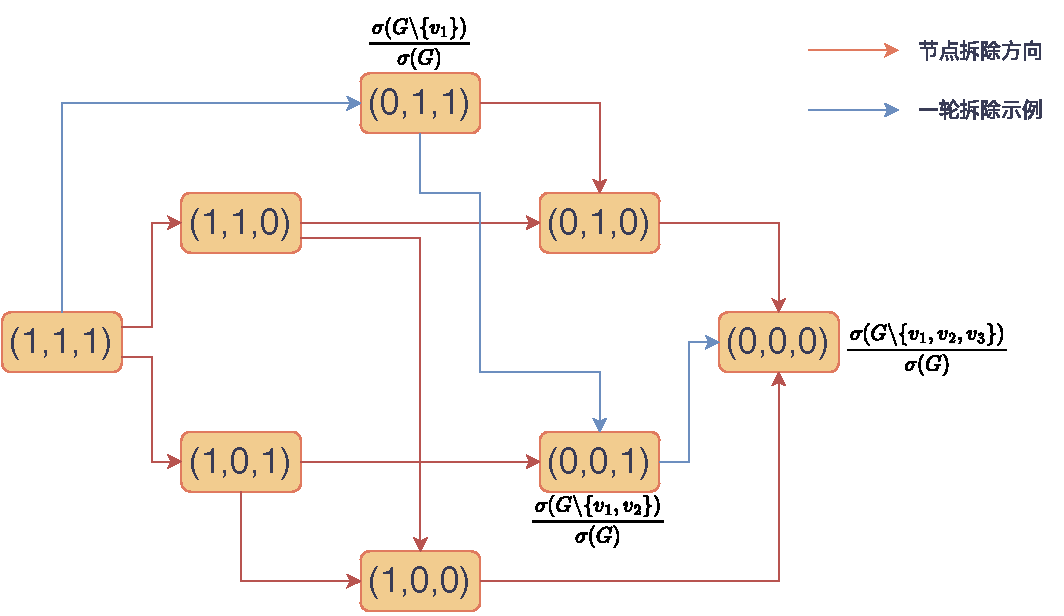
\includegraphics[width=0.49\textwidth]{网络状态转移图.pdf}
    \caption{节点数为3的网络状态转移图}
    \label{fig:网络状态转移图}
\end{figure}

节点的断连价值可以理解为断连前后状态连接性的差值,并非是一个定值,会随着状态的改变而改变。
由于网络拆解过程中网络连接性是单调不增的,因而最佳拆除策略是迭代拆除当前状态下断连价值最大的节点。

\begin{figure}[ht]
    \centering
    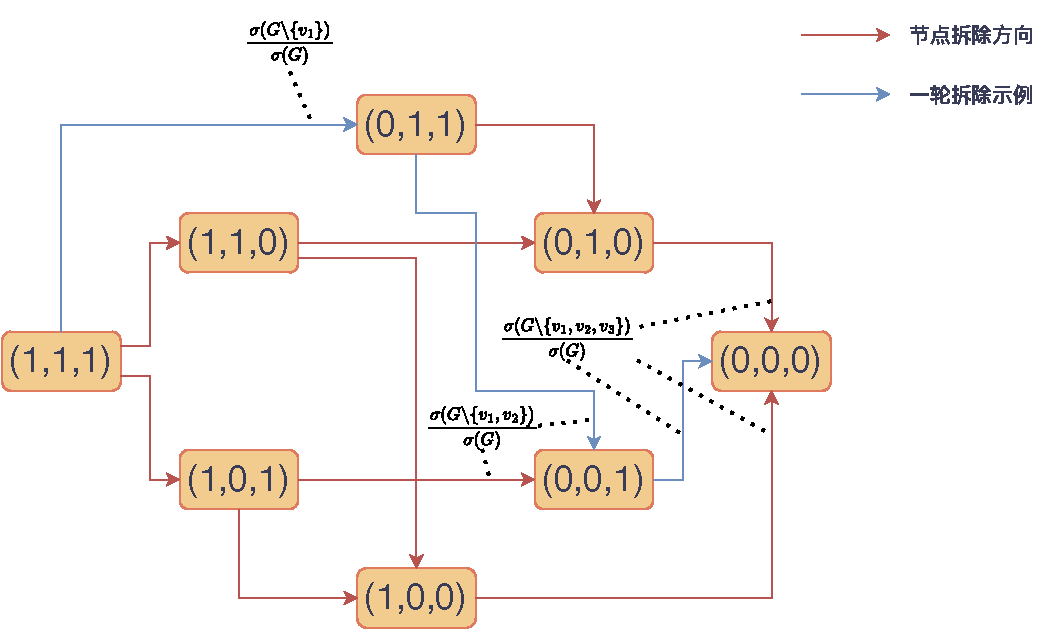
\includegraphics[width=0.49\textwidth]{最短路径问题.pdf}
    \caption{节点数为3对应的最短路径问题}
    \label{fig:最短路径问题}
\end{figure}

根据评价指标的定义及相关推论,显然有以下朴素算法成立:
针对特定的$\sigma$,计算每个状态的连接性,并将其转化为状态转移图中指向该状态的连边权重,
这样就将累积归一化连接性的最小化问题就可以转化为状态转移图从原始状态到全断连状态的最短路径问题(如图\ref{fig:最短路径问题}),
所求的最短路径就是最佳拆除策略,也就是在当前连接性指标$\sigma$下的最准确的节点影响力排序。


然而,这一朴素算法虽然能够在当前的评价指标下求出准确的节点影响力排序,
但由于其指数级的状态数,使得该算法只适用于小型图,而在面对大型图时面临严重的计算复杂度挑战。
因此,需要探索出一种在计算复杂度显著降低的前提下,依然能够保持良好准确度的算法。

\subsection{算法框架}\label{sec:AlgorithmFramework}

\begin{figure}[hptb]
    \centering
    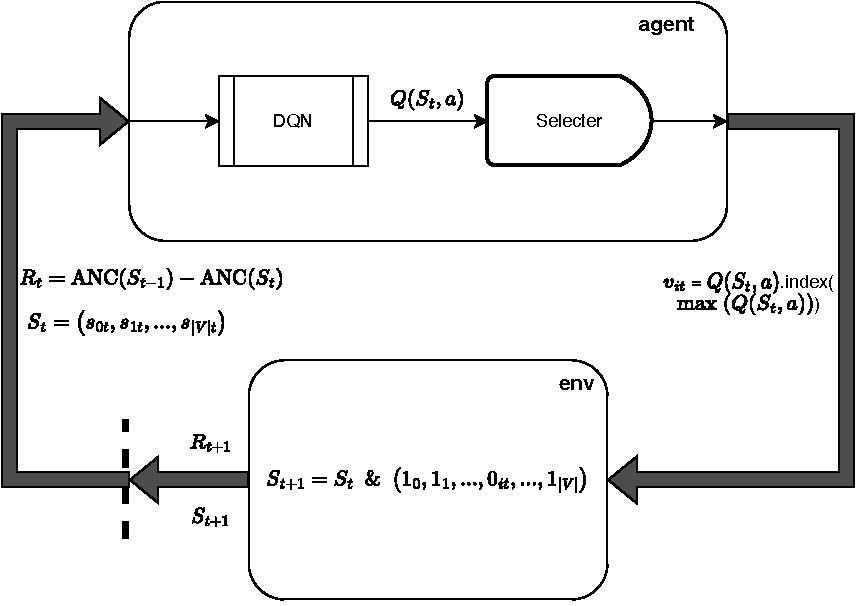
\includegraphics[width=0.49\textwidth]{算法框架图.pdf}
    \caption{算法框架图}
    \label{fig:算法框架图}
\end{figure}

通过前述分析,我们可以明显感知到,朴素算法所面临的计算复杂度局限性主要源自每个状态下节点断连价值的低效计算。
因此,本研究通过构建基于深度Q学习的强化学习模型来评估每个状态下各节点的断连价值,从而有效提升节点断连价值的计算效率。
在此基础上,运用贪心策略迭代断连断连价值最大的节点直至网络拆解结束,所得的断连顺序就是节点的影响力排序。

这一算法的核心原理如图\ref{fig:算法框架图}所示。其中,$S_t$表示网络$t$时刻的状态;
$v_{it}$表示$t+1$时刻agent决定断连的节点,由DQN输出的状态动作价值函数$Q(S_t, a)$确定;
$t$时刻的奖励$R$等于$t-1$时刻和$t$时刻ANC的差值。


\subsection{模型设计}\label{sec:ModelDesign}

本文为了提升模型模型收敛速度与泛化能力,将卷积神经网络中常用的迁移学习引入图神经网络中,把模型的离线训练过程分为基于排序学习的预训练过程和基于强化学习的训练过程。
相应的,根据用途将本文的神经网络模型分为三层,分别是嵌入层(Embedding Layer)、排序层(Ranking Layer)和评估层(Valuing Layer),如图\ref{fig:模型设计图}所示。

% \begin{figure}[htbp]
    \centering
    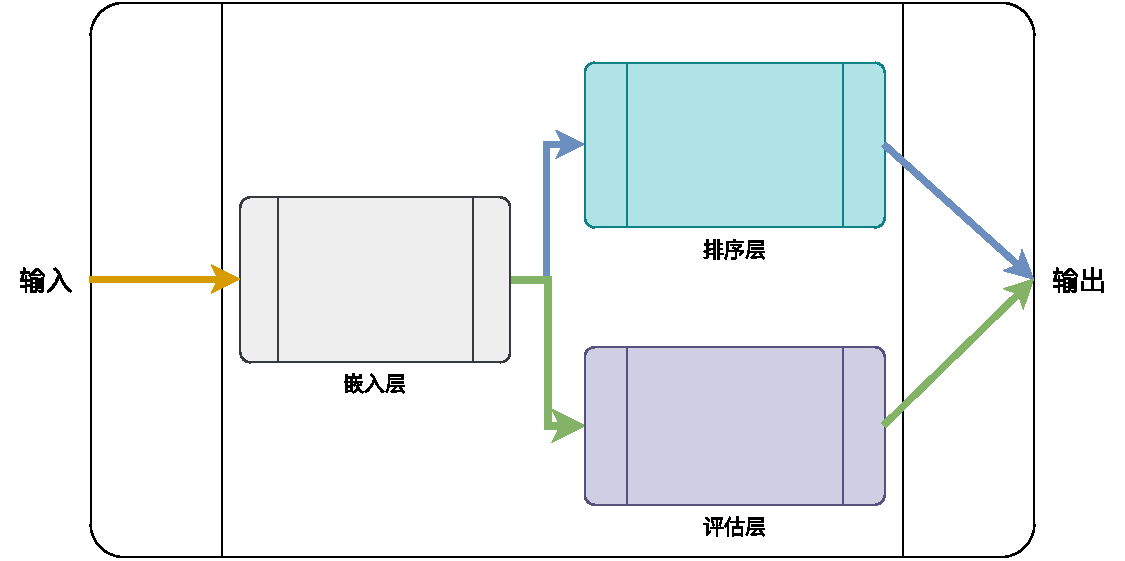
\includegraphics[width=0.49\textwidth]{模型设计图.pdf}
    \caption{模型设计图}
    \label{fig:模型设计图}
\end{figure}
\begin{figure*}[htbp]
    \centering
    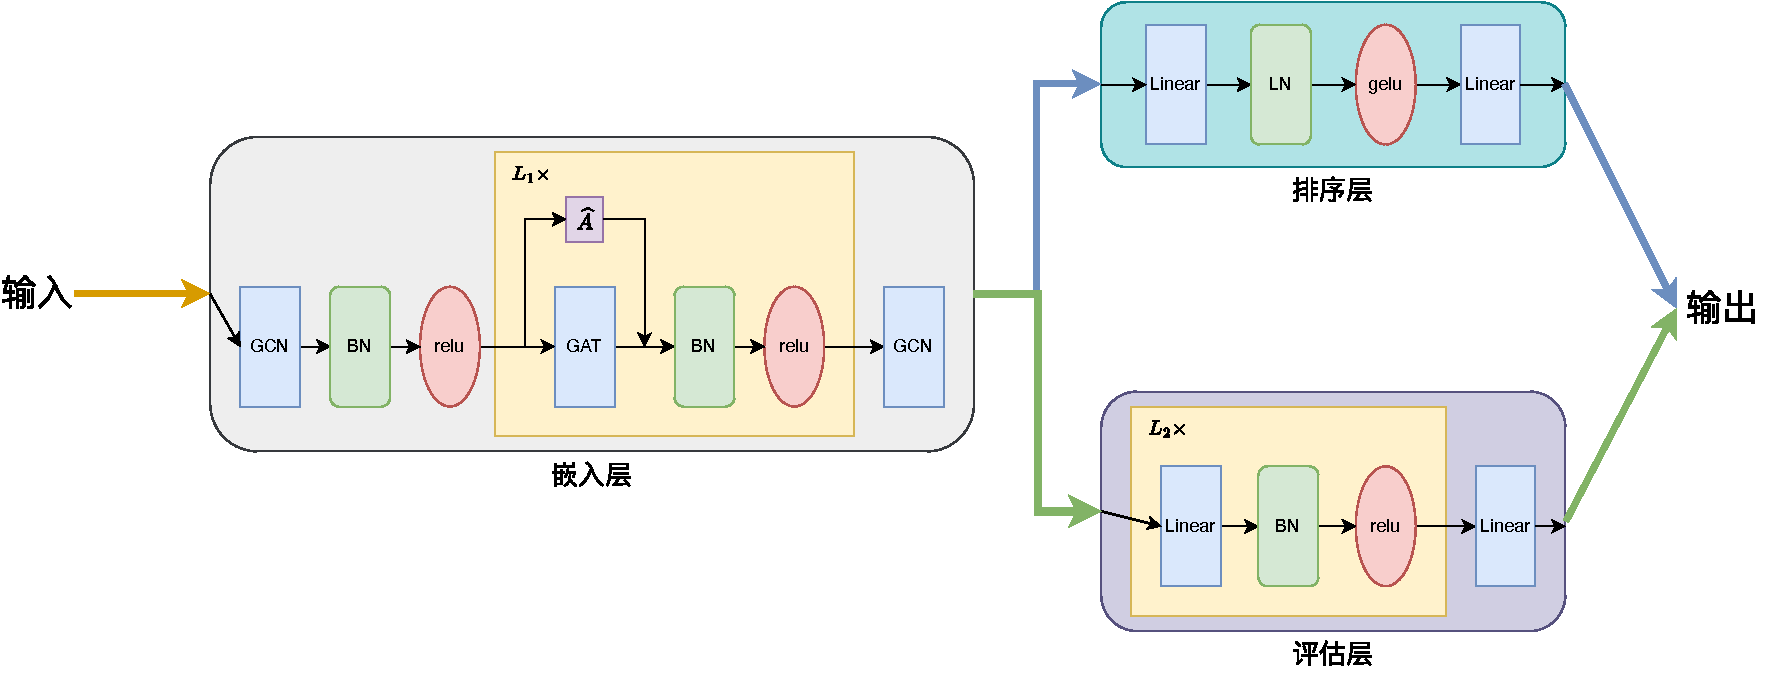
\includegraphics[width=1\textwidth]{模型设计图(总).pdf}
    \caption{模型设计图}
    \label{fig:模型设计图}
\end{figure*}

其中,排序学习预训练过程会利用到嵌入层和排序层并更新这两层的参数,而强化学习训练过程则会使用嵌入层和评估层,但会冻结嵌入层,只更新评估层的参数。
排序学习预训练具体流程会在\ref{sec:RankingLayer}节介绍,而强化学习训练具体过程会在\ref{sec:ValuingLayer}节介绍。


\subsubsection{模型嵌入层设计}\label{sec:EmbeddingLayer}

% \begin{figure}[htbp]
    \centering
    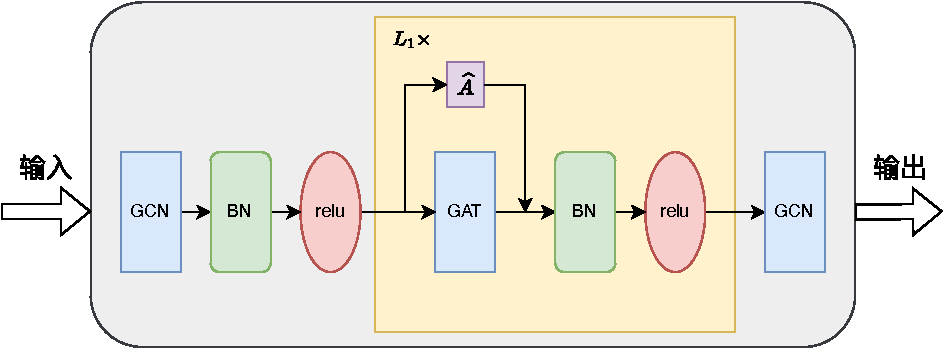
\includegraphics[width=0.49\textwidth]{嵌入层设计图.pdf}
    \caption{嵌入层设计图}
    \label{fig:嵌入层设计图}
\end{figure}

嵌入层主要起到特征提取的作用,输入一个或多个图数据所构成的数据批,包含相应的邻接矩阵$A$和特征矩阵$X$,
输出节点的图嵌入向量。

通过引入图残差网络\cite{zhang2019GResNet}(Graph Residual Network, GResNet)中的graph-naive residual残差块,
让模型更好地捕捉图中节点之间的复杂关联,从而克服深度谱域图神经网络假死问题(Suspended Animation Problem):
\begin{equation}
    \mathrm{R}\left(k; \mathcal{G}\right)=\hat{\mathbf{A}} \mathbf{H}_{k}, 
    \forall k \in \{ 1, 2,... L_1 \}
    \label{formula:残差块表达式}
\end{equation}
\noindent 其中,$L_1$表示残差块的数量,$\mathbf{H}_{k}$代表第$k$个残差块的输入,$\hat{\mathbf{A}}$代表输入网络$\mathcal{G}$的归一化邻接矩阵($\hat{\mathbf{A}} = \mathbf{D}^{-\frac{1}{2}}(\mathbf{A}+\mathbf{I}) \mathbf{D}^{-\frac{1}{2}}$)。

每个残差块中都使用结合图注意力机制的GAT卷积层,满足:
\begin{equation}
\vec{h_i^\prime}=\sigma\left(\sum_{v_j \in \mathcal{N}\left(v_i\right)} \alpha_{i j} W \vec{h_j}\right)
\label{formula:GATConv}
\end{equation}
\noindent 其中,激活函数$\sigma$选用ReLU,$\vec{h_i}$、$\vec{h_i^\prime}$分别表示GAT卷积层中第$i$个节点的输入、输出特征,
而$\alpha_{ij}$代表节点$v_i$与节点$v_j$之间的注意力权重,可以表示为:
\begin{equation}
    \alpha_{ij} = \frac{\exp(\operatorname{LeakyReLU}(\vec{a}^{T} (\mathbf{W}\vec{h_i} \cdot \mathbf{W}\vec{h_j})))}
    {\sum_ {v_k\in N(v_i)} \exp(\operatorname{LeakyReLU}(\vec{a}^T (\mathbf{W}\vec{h_i} \cdot \mathbf{W}\vec{h_k}))) }
    \label{formula:影响力权重}
\end{equation}

此外,通过在卷积层后添加批归一化(Batch Normalization, BN),可以减小训练过程中的内部协变量偏移(Internal Covariate Shift)问题,
从而使得网络对输入数据的变化更加稳定,从而加速模型的训练收敛过程。

根据式\ref{formula:残差块表达式}、式\ref{formula:GATConv}和式\ref{formula:影响力权重},结合嵌入层的其他组件,
可以算出节点的图嵌入向量可以用以下方程表示:

\begin{equation}
	\begin{cases}
	\mathbf{H}_{1} & =\sigma\left(\operatorname{BN}\left(\hat{\mathbf{A}} \mathbf{X}_\mathrm{I} \mathbf{W}_\mathrm{I}\right)\right) \\
	\mathbf{H}_{k+1} & = \sigma\left(\operatorname{BN}\left(\mathcal{F}_k\left(\mathbf{H}_{k} \right) + \hat{\mathbf{A}} \mathbf{H}_{k}\right)\right), k \in [1, L_1-1] \\
	\mathbf{X}_\mathrm{O} & = \hat{\mathbf{A}}\left(\sigma\left(\operatorname{BN}\left(\mathcal{F}_{L_1}\left( \mathbf{H}_{L_1} \right) + \hat{\mathbf{A}} \mathbf{H}_{k}\right)\right)\right) \mathbf{W}_\mathrm{O}
	\end{cases}
    \label{formula:嵌入层特征矩阵方程}
\end{equation}


\noindent 其中,
$\mathcal{F}_k$是一个基于GAT卷积层中线性权重矩阵$\mathbf{W}_k$和注意力权重向量$\vec{a_{k}}$的函数,
$W_\mathrm{I}$和$W_\mathrm{O}$分别代表残差串前后GCN卷积层的权重,
$\mathbf{X}_{I}$表示嵌入层/整个模型的输入特征矩阵,而$\mathbf{X}_{O}$表示嵌入层的输出特征矩阵。

\subsubsection{模型排序层设计}\label{sec:RankingLayer}
排序层的作用是对节点影响力作文档对(Pairwise)方法的排序学习,
其输入矩阵$Y_\mathrm{I}$由嵌入层输出矩阵$\mathbf{X}_\mathrm{O}$的每个节点特征向量的笛卡尔积构成,可以表示为:

\begin{equation}
    \vec{y_k} = \vec{x_i} \| \vec{x_j}, \quad \forall i \in [1, |V|], j \in [1, |V|]
    \label{formula:排序层输入}
\end{equation}

\noindent 其中,$x_i$、$x_j$是$\mathbf{X}_\mathrm{O}$中的行向量。相应的,将训练集也做类似的处理。

% \begin{figure}[htb]
    \centering
    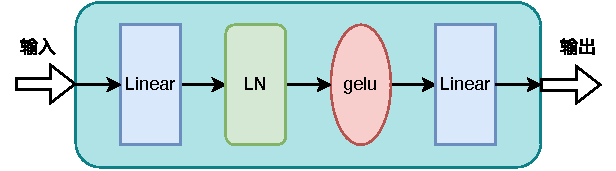
\includegraphics[width=0.49\textwidth]{排序层设计图.pdf}
    \caption{排序层设计图}
    \label{fig:排序层设计图}
\end{figure}

排序层内部通过双层的MLP实现对输入特征向量的二分类,当输出高于阈值时,预测$x_i$所对应的节点$v_i$的影响力高于$x_j$对应的节点$v_j$,反之同理。
之后,将预测值与真实值做均方差后反向传播更新模型。


\subsubsection{模型评估层设计}\label{sec:ValuingLayer}

本文中的评估层近似于一个完整的DQN,
输入嵌入层得到的特征矩阵$X_E$,它可以看作是当前网络的状态$S_t$,
输出则是当前状态下网络中任意节点的断连价值。

% \begin{figure}[htbp]
    \centering
    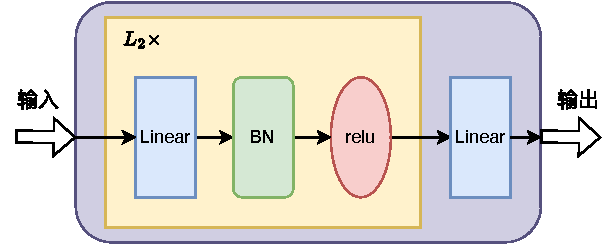
\includegraphics[width=0.49\textwidth]{评估层设计图.pdf}
    \caption{评估层设计图}
    \label{fig:评估层设计图}
\end{figure}

考虑到网络状态的特征提取已在嵌入层中实现,因此评估层只需要$L_2$层MLP处理剩余的回归问题即可。


\section{实验评估}\label{sec:ExperimentalEvaluation}

\subsection{数据来源}\label{sec:DataCollection}

本文所使用的数据集可以分为两种,一种是用于训练模型的合成数据集,另一种是用于验证模型的真实数据集。


\subsubsection{合成数据集}\label{sec:SyntheticDataset}

合成数据集的构建分为三个步骤:生成原始网络、计算节点特征、获取排序标签

首先使用erdos renyi(ER)、small world(SW)、barabasi albert(BA)三种网络模型分别生成随机网络、小世界网络和无标度网络。
生成过程中,只需控制网络的节点数和平均度两个参数,
将节点数$|V|$分为六个区间,分别是30-50、50-100、100-200、200-300、300-400和400-500,
并让平均度$k$满足式\ref{formula:合成网络的平均度分布}的powerlaw分布,对每种模型的每个度区间都随机生成100个网络实例。

% https://gizapedia.org/static/786bb254b9f75741600fc9ca31fcde81/english_beamer_powerlaw.pdf

\begin{equation}
    % f(x)=\frac{\alpha-1}{x_{\min }}\left(\frac{x}{x_{\min }}\right)^{-\alpha} ; x>x_{\min } ; \alpha>1
    f(k_\mathrm{avg})=\frac{\alpha-1}{\Gamma}\left(\frac{k_\mathrm{avg}}{\Gamma}\right)^{-\alpha} ; k_\mathrm{avg} > \Gamma ; \alpha>1
    \label{formula:合成网络的平均度分布}
\end{equation}



然后,选取DC、K-Core、HITS分别代表网络中节点的邻域信息、拓扑结构和特征向量三个方面的属性,为每个网络构建一个$|V|\times3$的特征矩阵。

最后,选用在复杂度和准确度上表现均衡的PageRank算法作为原始节点影响力排序算法,获取节点的排序标签。


\subsubsection{真实数据集}\label{sec:RealDataset}

\begin{table*}[hpbt]
    \centering
    \begin{tabular}{cccccccc}
    \thickhline
    网络名称 &   网络类别   & $|V|$ & $|E|$ & $k_{\mathrm{avg}}$ & $d_{\mathrm{avg}}$ &  $d_{\mathrm{max}}$ & $\ln |V|/\ln k_\mathrm{avg}$ \\
    \hline
    karateclub&   社交    &   34                  &         78            &      4.588                       &      2.408                       &         5                         &           2.315            \\
    email   &     社交    & 1005                  &      16064            &     31.968                       &      2.587                       &         7                         &           1.995            \\
    bible   &     信息    & 1773                  &       9131            &     10.300                       &      3.375                       &         8                         &           3.208            \\
    % coraml  &     信息    & 2995                  &       8158            &      5.448                       &      5.271                       &        17                         &           4.722            \\
    airport &     交通    & 1190                  &      13599            &     22.855                       &      3.069                       &         8                         &           2.263            \\
    euroroad&     交通    & 1174                  &       1417            &      2.414                       &     18.395                       &        62                         &           8.020            \\
    % amazon  &     经济    & 7647                  &     119081            &     31.145                       &      4.051                       &        11                         &           2.600            \\
    beacxc  &     经济    &  493                  &      42176            &    171.099                       &      1.652                       &         3                         &           1.206            \\
    diseasome&    生物    &  516                  &       1188            &      4.605                       &      6.509                       &        15                         &           4.090            \\
    % protein &     生物    & 4182                  &      13115            &      6.272                       &      4.090                       &        11                         &           4.541            \\
    \thickhline
    \end{tabular}
    \caption{真实数据集结构表}
    \label{table:真实数据集结构表}
\end{table*}

为了验证模型的泛化能力和实用性,本文选取了来自交通网络、经济网络、信息网络、生物网络以及社交网络的共7个真实数据集。
统计特征如表\ref{table:真实数据集结构表}所示,
$|V|$为节点数,$|E|$为边数,$k_{\mathrm{avg}}$为平均度,$d_{\mathrm{avg}}$为最大连通子图的平均距离,$d_{\mathrm{max}}$为最大连通子图的直径,$\ln |V|/\ln k_\mathrm{avg}$为无标度性参数。
所有网络都可以从Network Repository\footnote{https://networkrepository.com/}、PyG Datasets\footnote{https://pytorch-geometric.readthedocs.io/}和KONECT\footnote{http://konect.cc/}中获取。
实验过程中将这些真实网络均视为无权无向图。


\subsection{结果分析}\label{sec:ResultAnalysis}

为了验证本文所提出的算法是否在准确度和复杂度上具有优势,选取了四种节点影响力评估算法进行了对比,分别是
HDA\cite{cohen2001HDA}、CI、K-Core、PageRank。

\subsubsection{准确度}\label{sec:Accuracy}

首先在合成数据集上测试本文所提算法的准确度,结果如图\ref{fig:合成数据集-ANCBar}所示,
可以看出,本文所提出的算法在ER随机网络和SW小世界网络的场景下明显优于基线算法,在BA无标度网络的场景下准确度也较为理想。

之后在真实数据集上验证所提算法的泛化能力,部分真实网络在不同算法下剩余连通性与网络拆解比例的关系如图\ref{fig:真实数据集-ANCCurve}所示,
可以明显看出使用本文所提算法的曲线在网络拆解比例较小的时候相对基线算法有更高的下降速率,据此可以推断本文所提的算法将具有更好的准确度。
真实数据集上不同算法ANC数值(见表\ref{table:真实数据集-ANCTable})同样验证了这一结论。

% \begin{figure*}
%     \centering
%     \begin{subfigure}{0.48\textwidth}
%         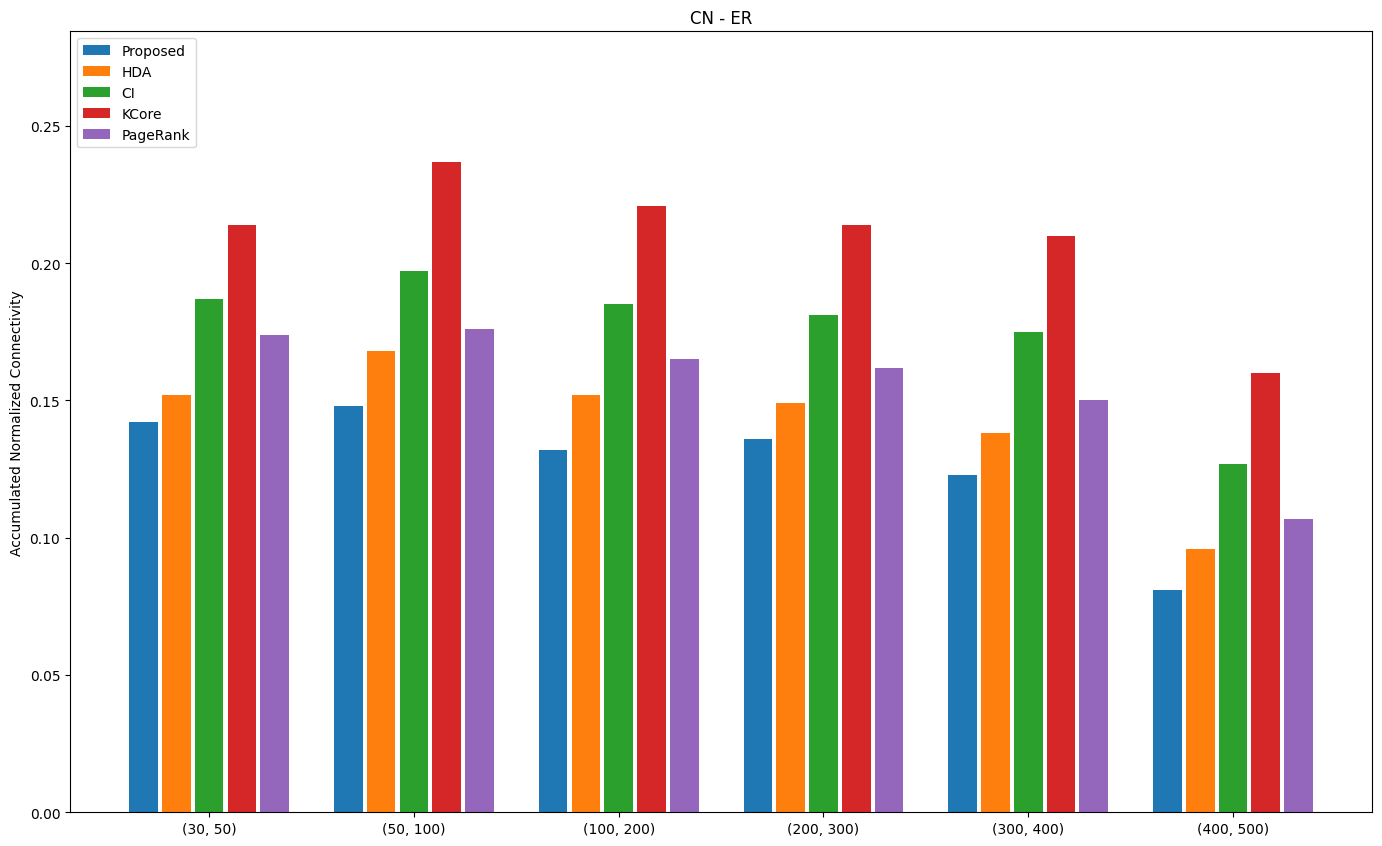
\includegraphics[width=\linewidth]{ANC_CN_ER.png}
%         \caption{CN - ER}
%     \end{subfigure}%
%     \hfill
%     \begin{subfigure}{0.48\textwidth}
%         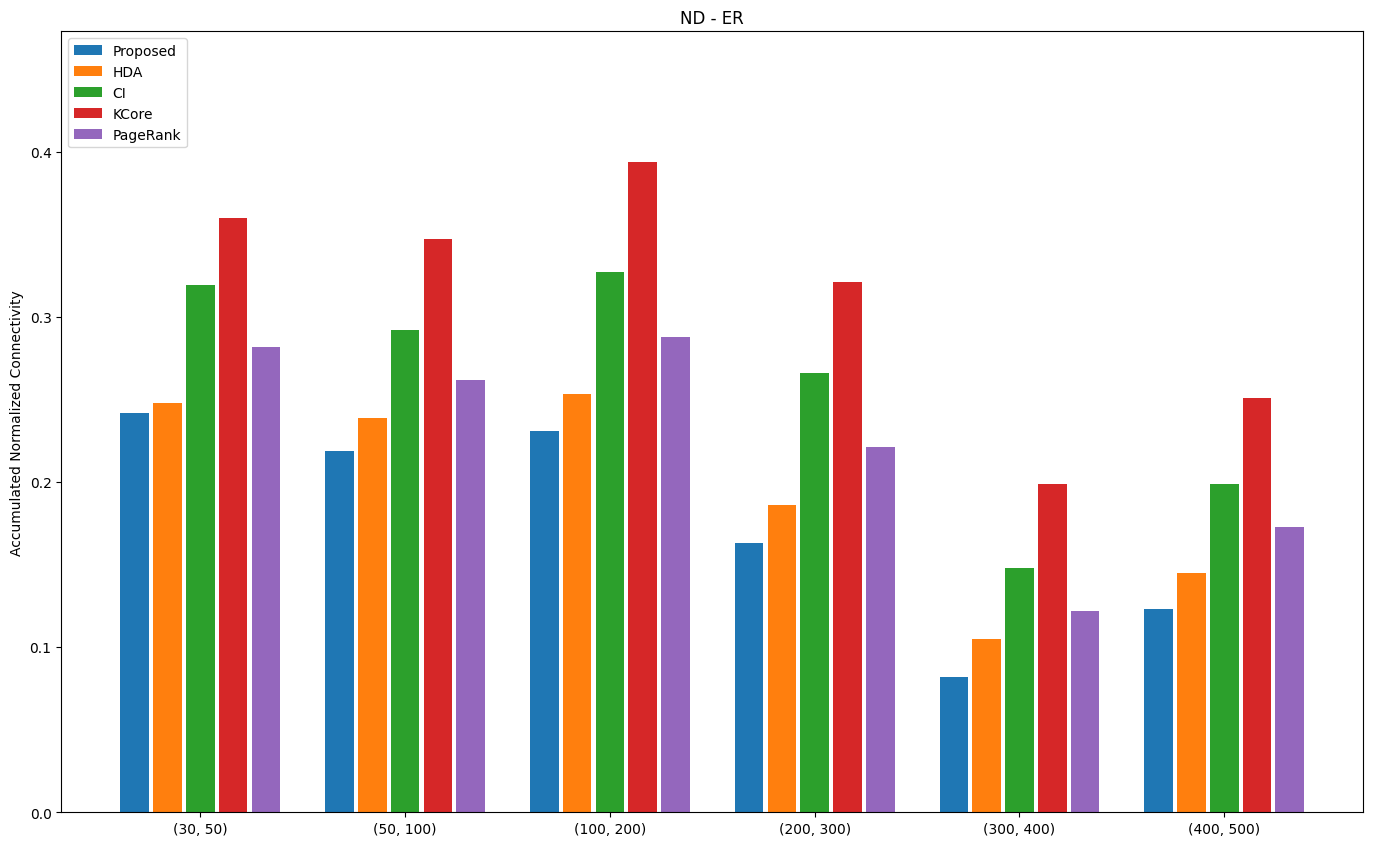
\includegraphics[width=\linewidth]{ANC_ND_ER.png}
%         \caption{ND - ER}
%     \end{subfigure}%

%     \medskip

%     \begin{subfigure}{0.48\textwidth}
%         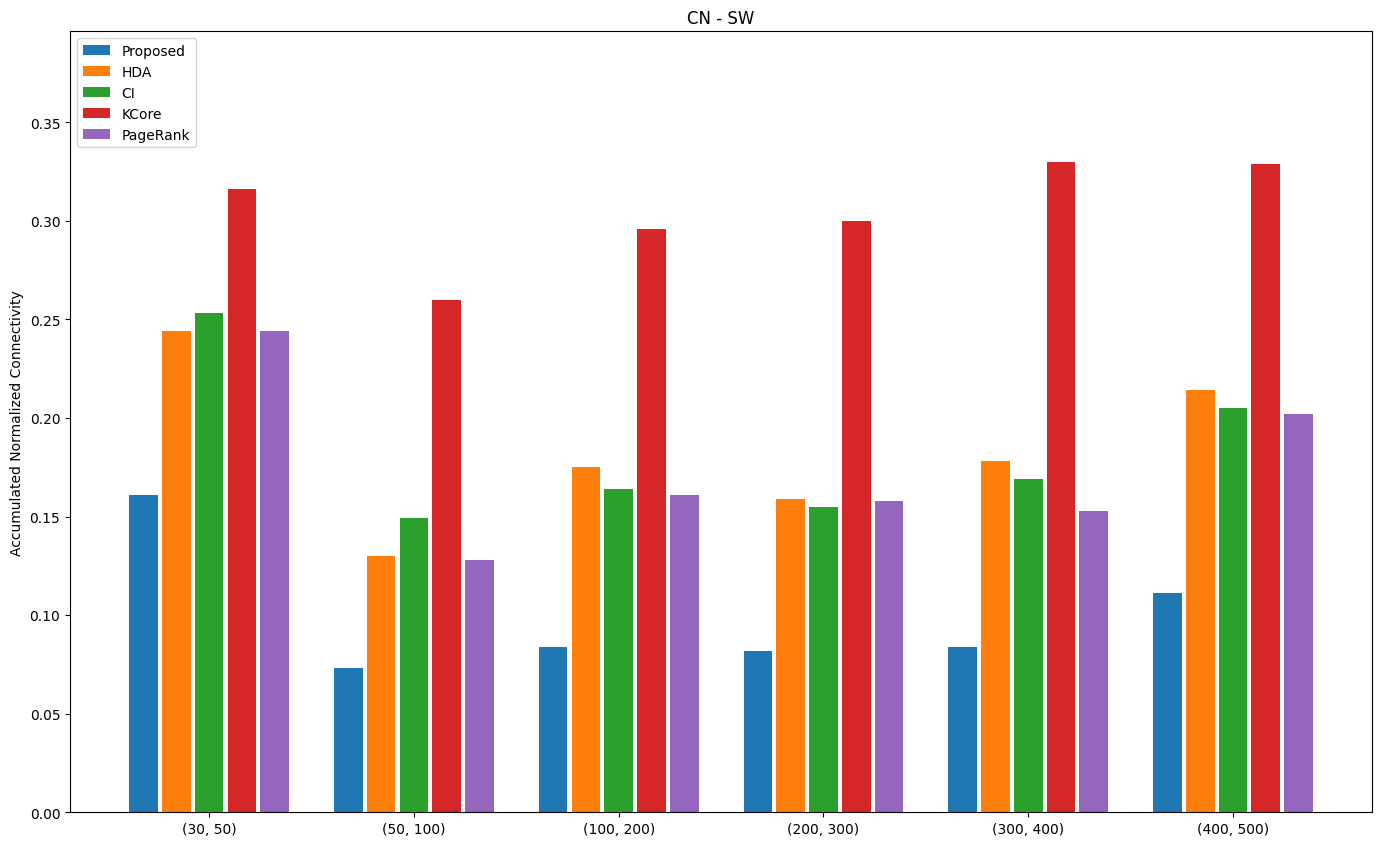
\includegraphics[width=\linewidth]{ANC_CN_SW.png}
%         \caption{CN - SW}
%     \end{subfigure}%
%     \hfill
%     \begin{subfigure}{0.48\textwidth}
%         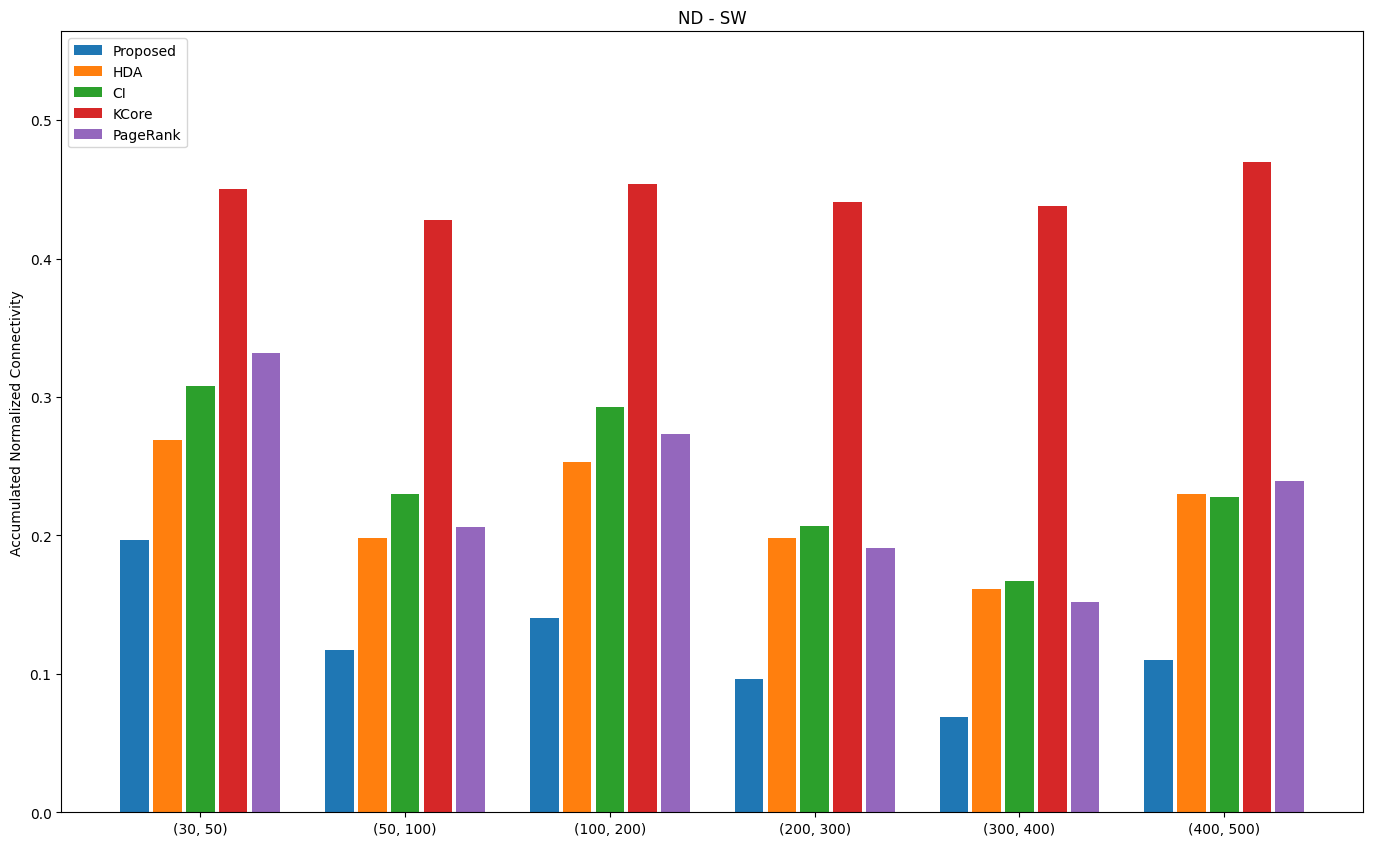
\includegraphics[width=\linewidth]{ANC_ND_SW.png}
%         \caption{ND - SW}
%     \end{subfigure}%

%     \medskip

%     \begin{subfigure}{0.48\textwidth}
%         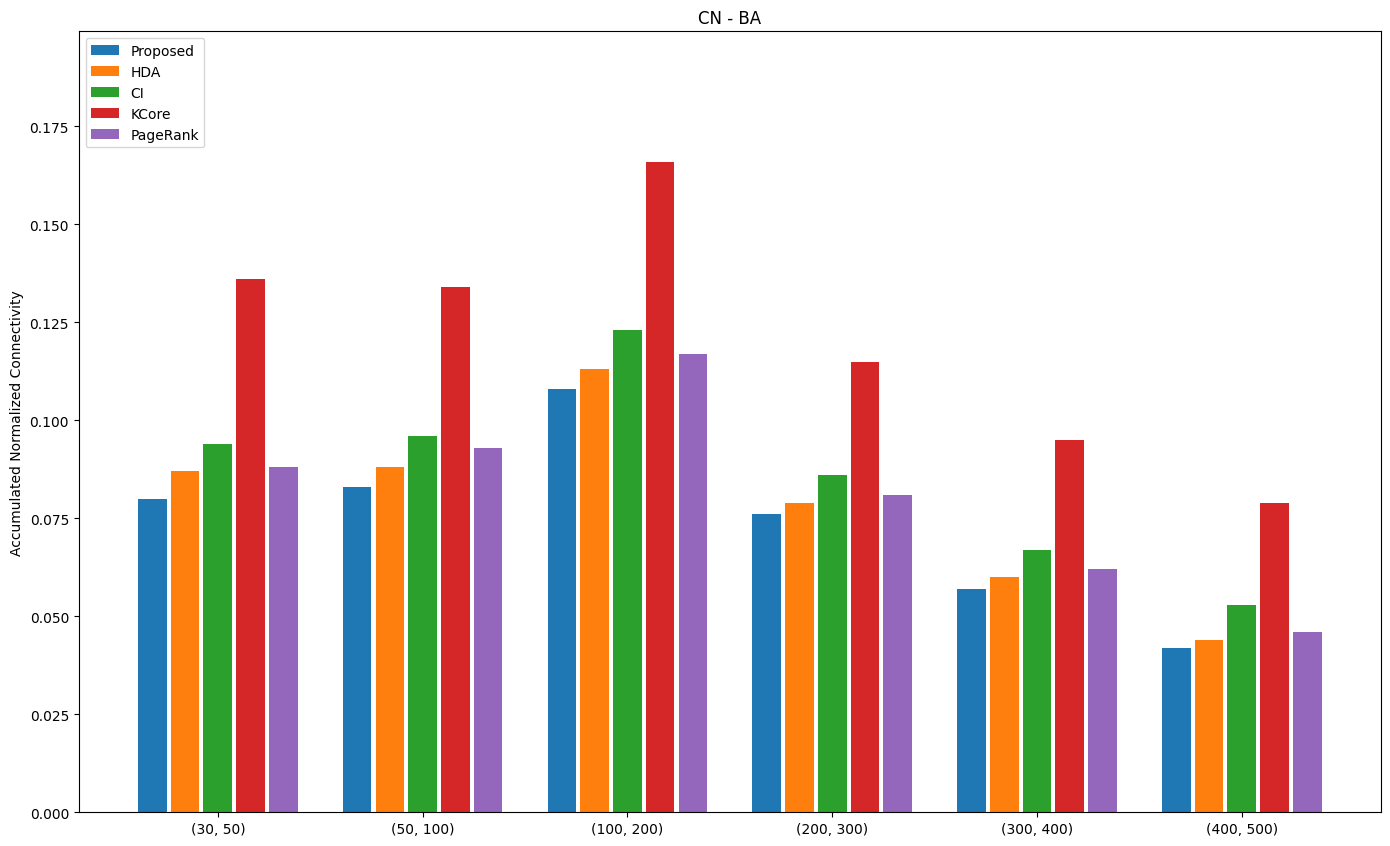
\includegraphics[width=\linewidth]{ANC_CN_BA.png}
%         \caption{CN - BA}
%     \end{subfigure}%
%     \hfill
%     \begin{subfigure}{0.48\textwidth}
%         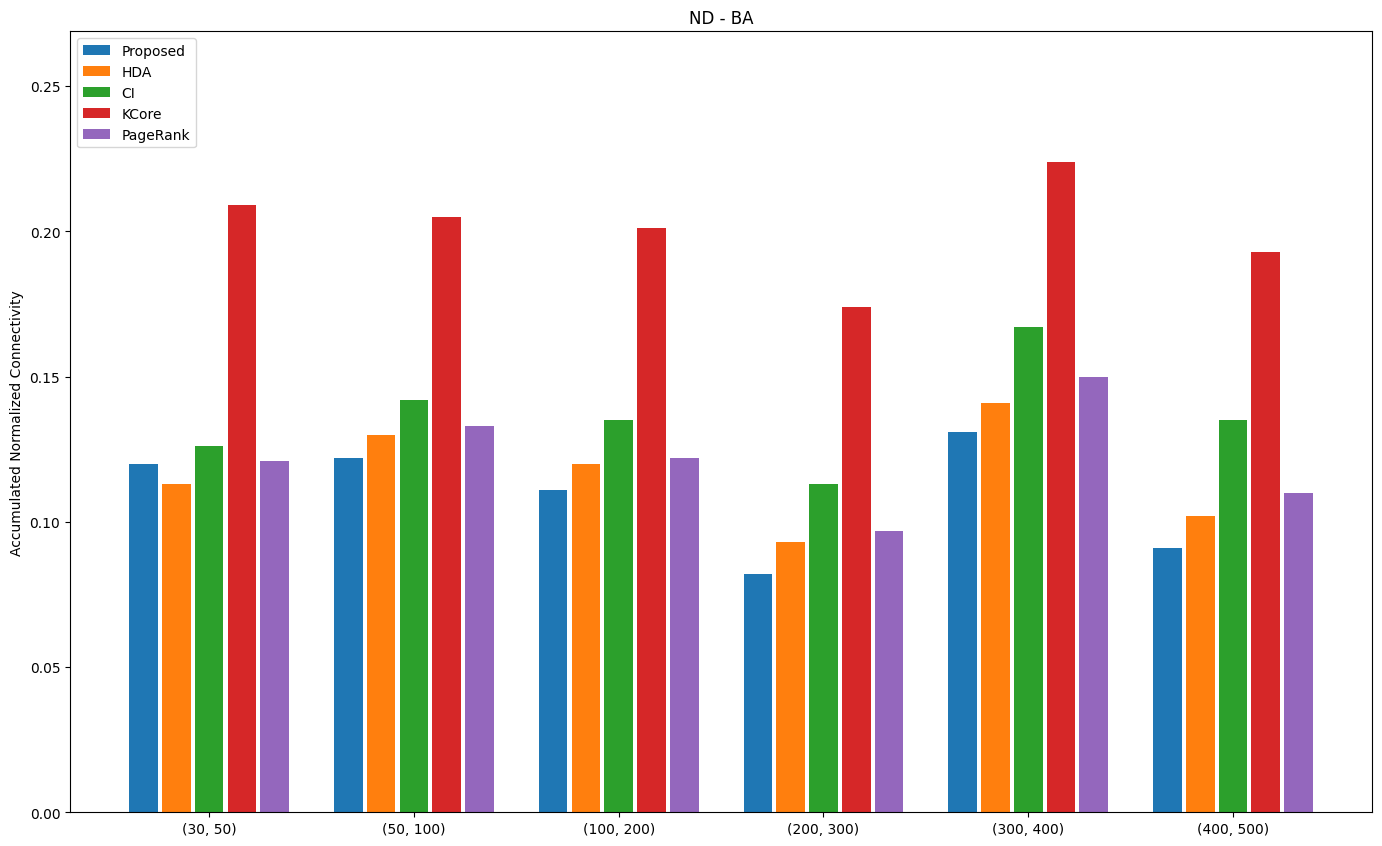
\includegraphics[width=\linewidth]{ANC_ND_BA.png}
%         \caption{ND - BA}
%     \end{subfigure}%
% \end{figure*}


\begin{figure*}[hptb]
    \centering
    \begin{subfigure}{0.32\textwidth}
        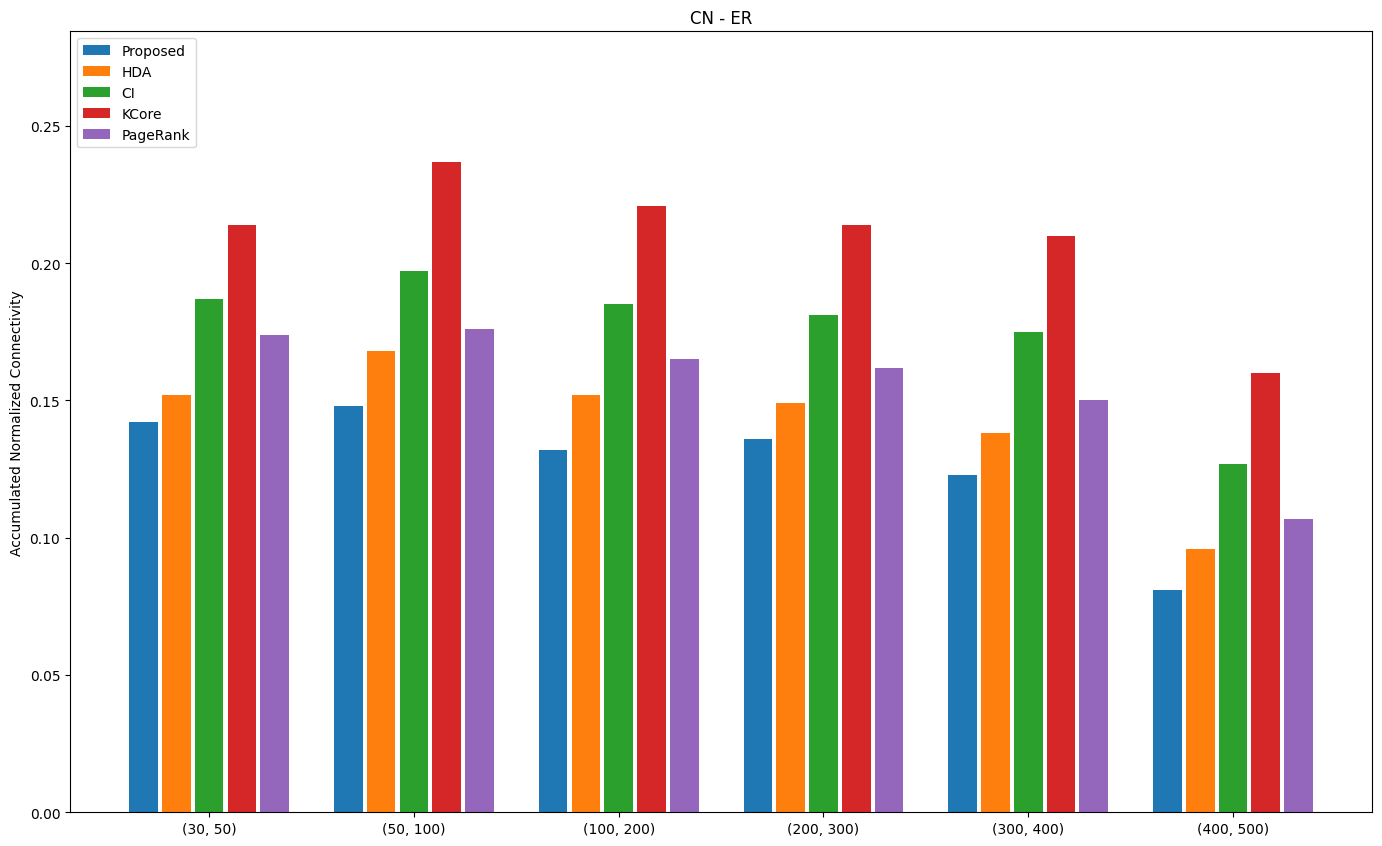
\includegraphics[width=\linewidth]{ANC_CN_ER.png}
        \caption{CN - ER}
    \end{subfigure}%
    \hfill
    \begin{subfigure}{0.32\textwidth}
        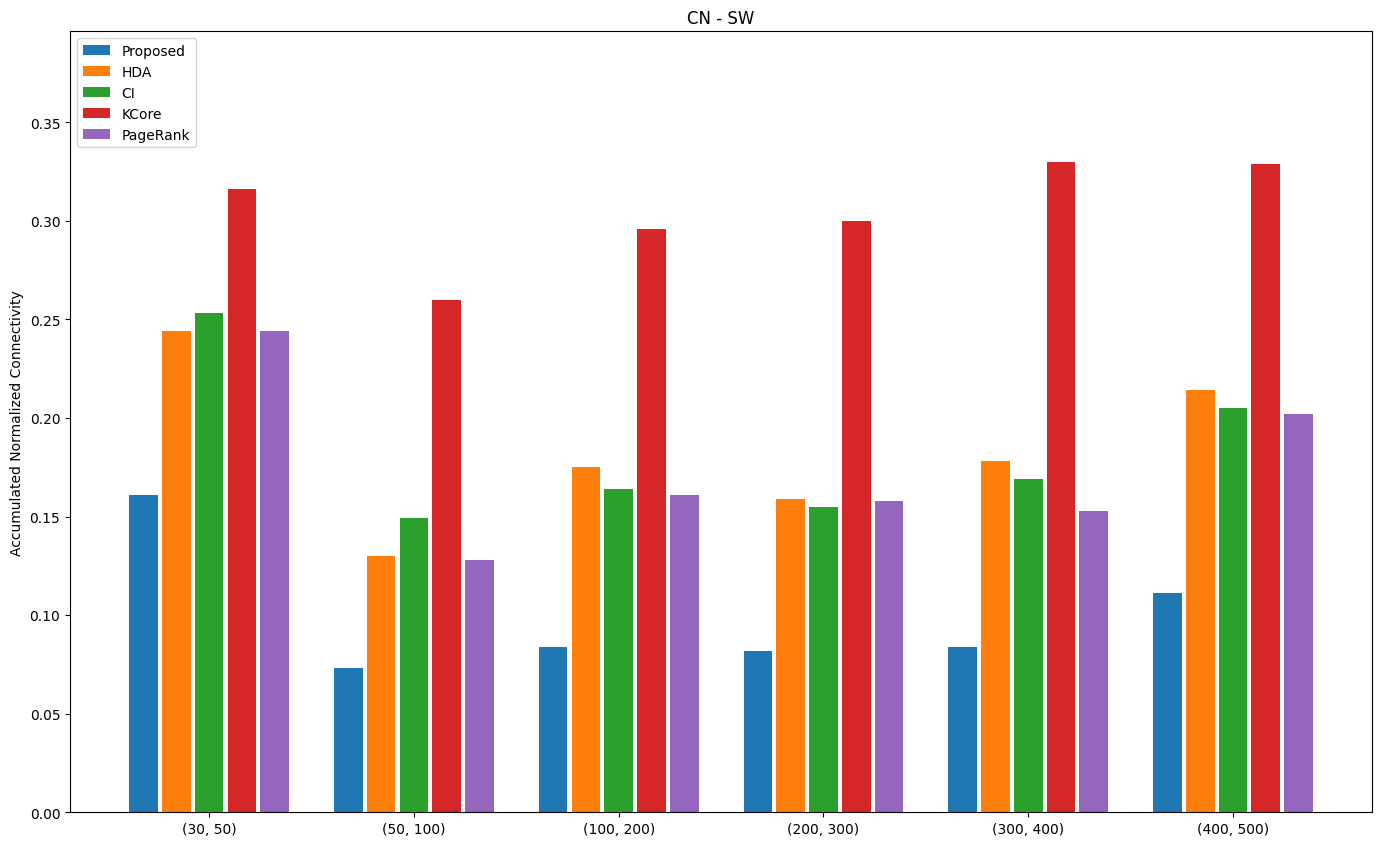
\includegraphics[width=\linewidth]{ANC_CN_SW.png}
        \caption{CN - SW}
    \end{subfigure}%
    \hfill
    \begin{subfigure}{0.32\textwidth}
        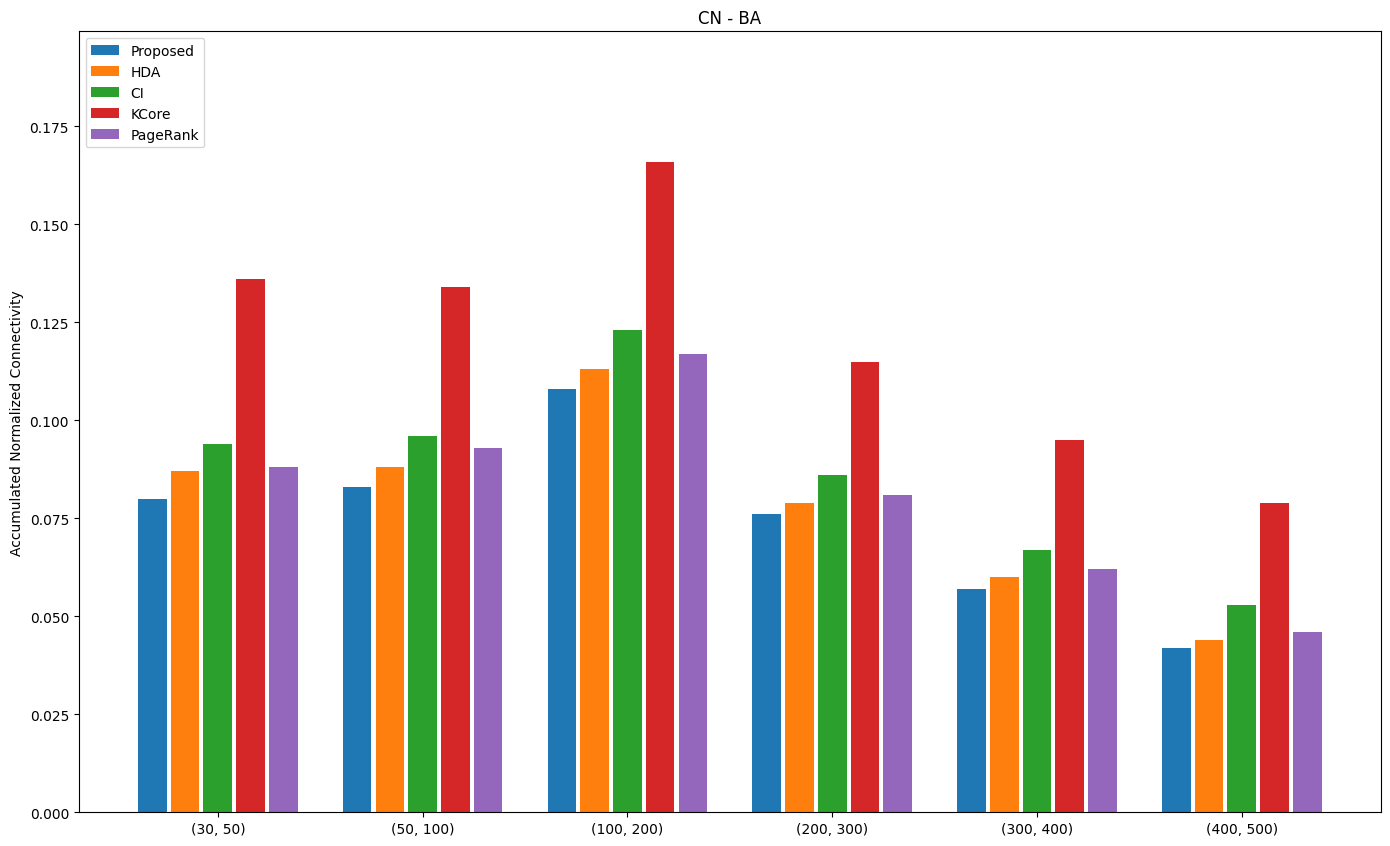
\includegraphics[width=\linewidth]{ANC_CN_BA.png}
        \caption{CN - BA}
    \end{subfigure}%

    \medskip

    \begin{subfigure}{0.32\textwidth}
        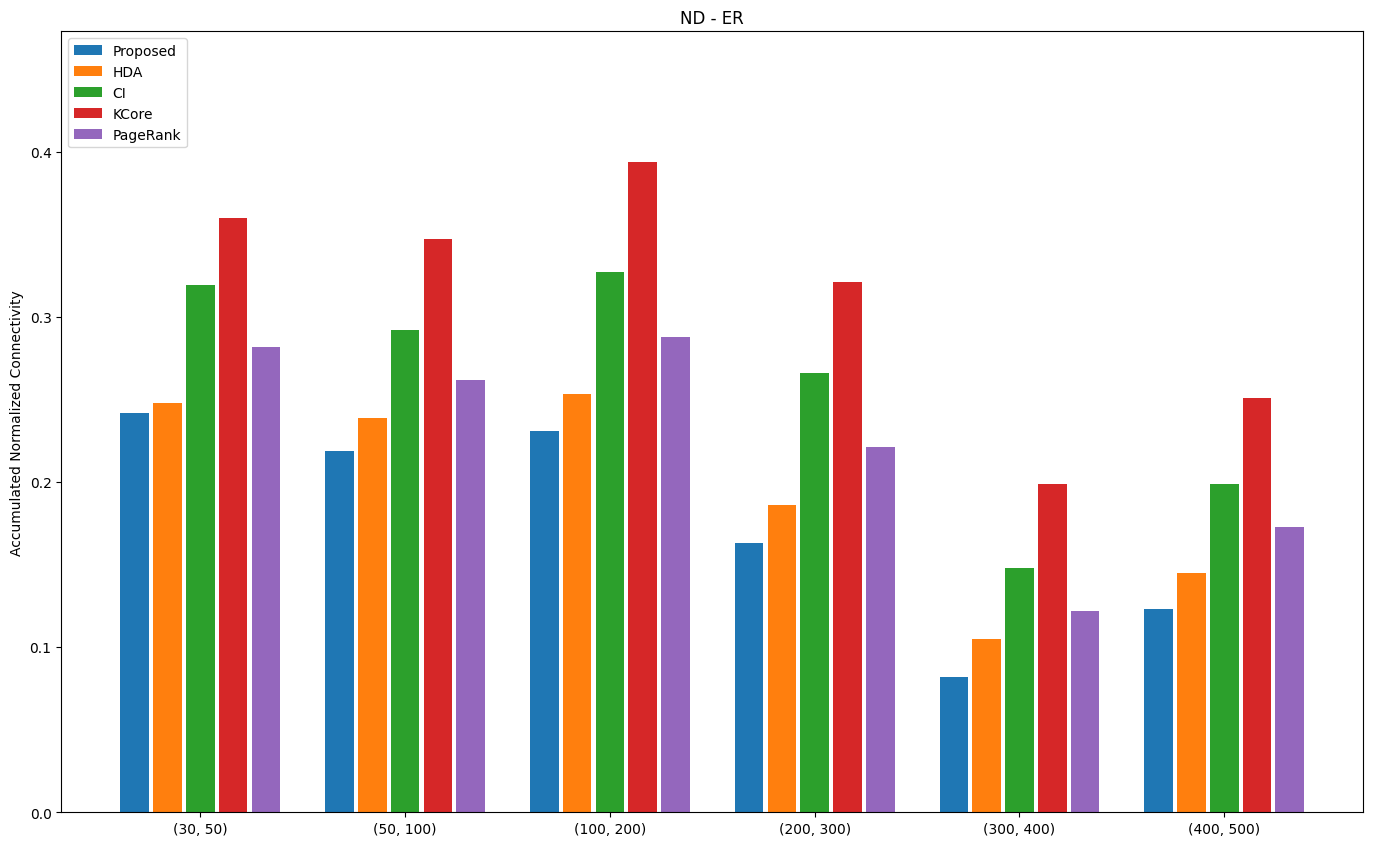
\includegraphics[width=\linewidth]{ANC_ND_ER.png}
        \caption{ND - ER}
    \end{subfigure}%
    \hfill
    \begin{subfigure}{0.32\textwidth}
        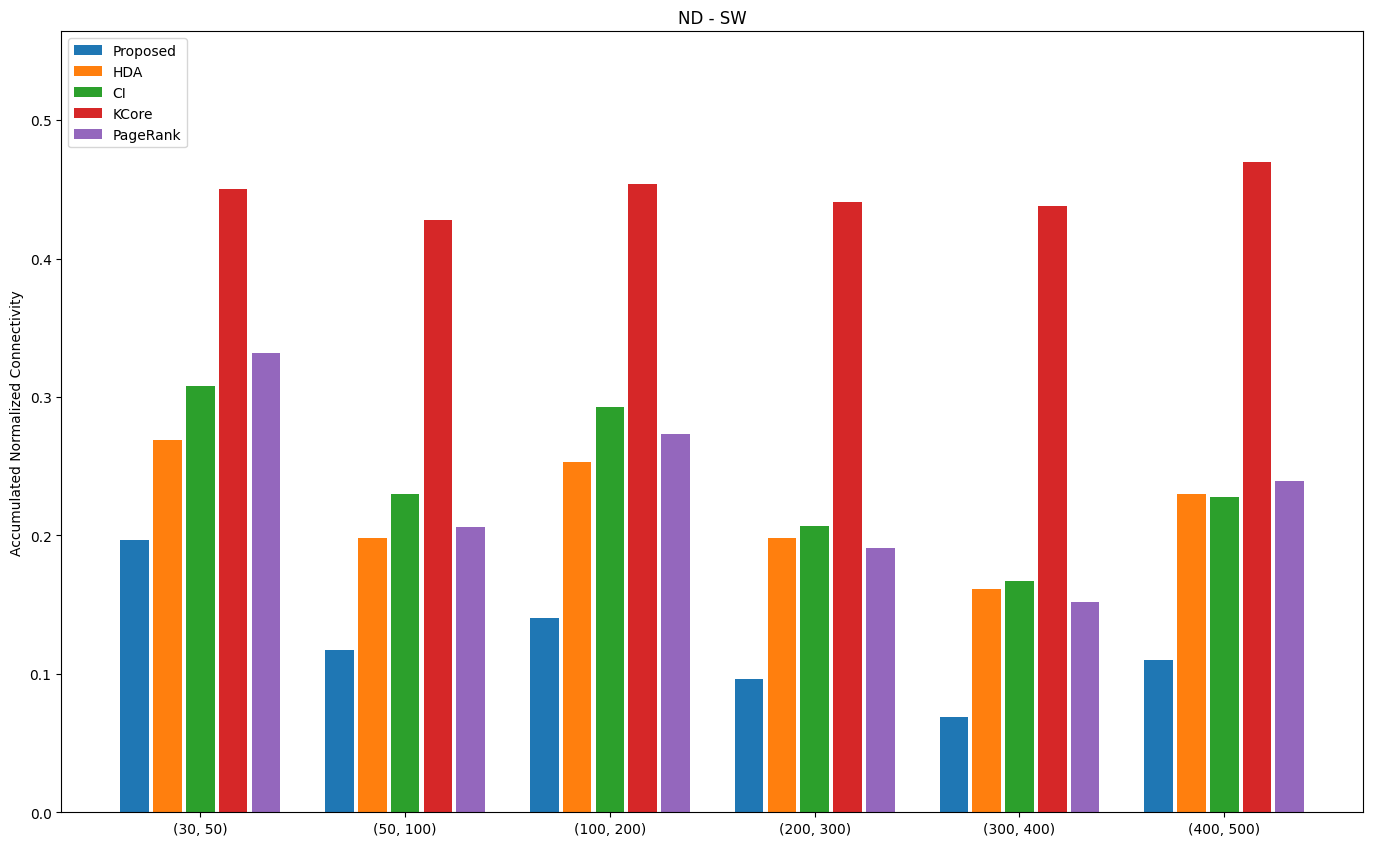
\includegraphics[width=\linewidth]{ANC_ND_SW.png}
        \caption{ND - SW}
    \end{subfigure}%
    \hfill
    \begin{subfigure}{0.32\textwidth}
        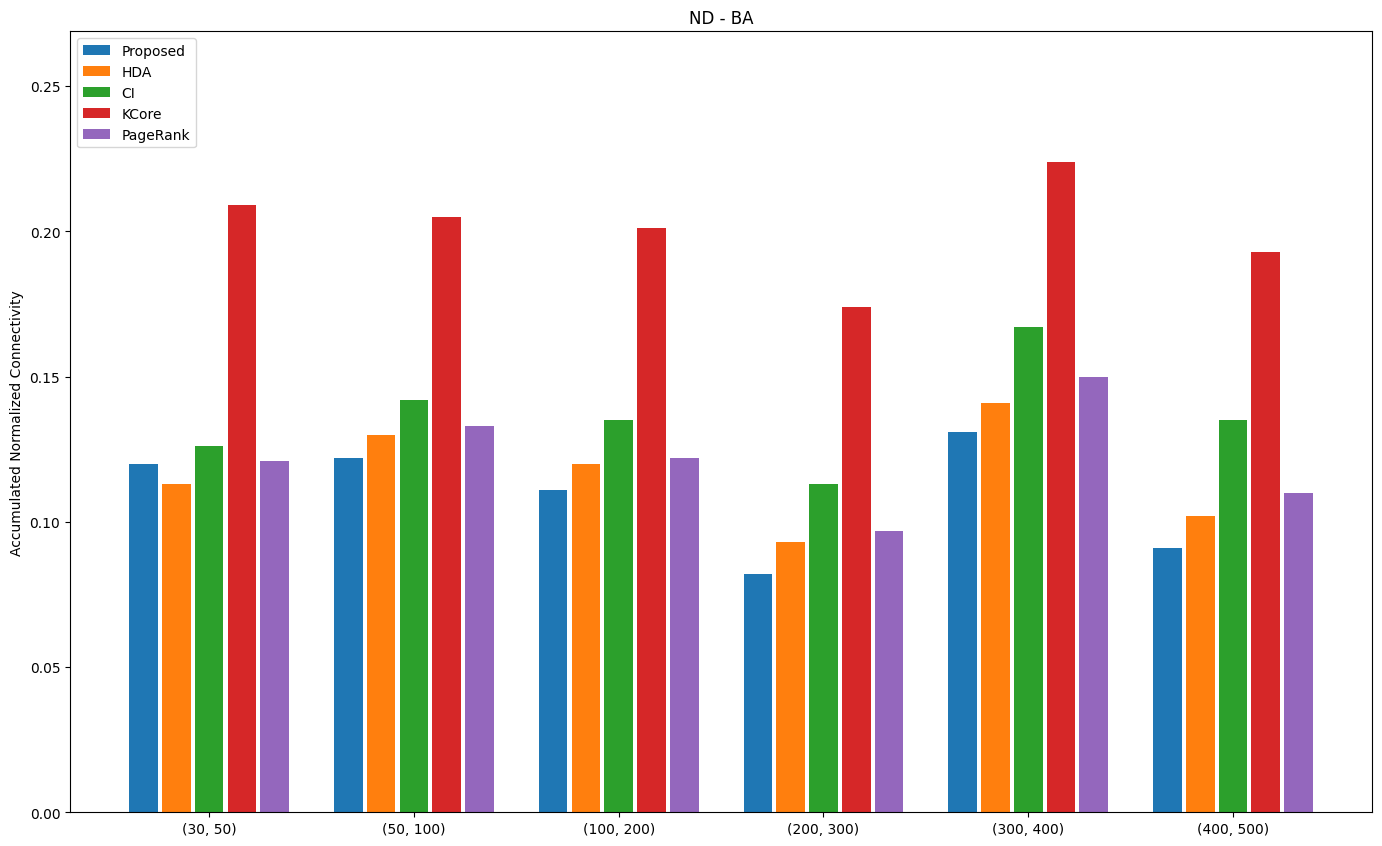
\includegraphics[width=\linewidth]{ANC_ND_BA.png}
        \caption{ND - BA}
    \end{subfigure}%
    \caption{合成数据集上不同算法在各节点数区间上的ANC均值}
    \label{fig:合成数据集-ANCBar}
\end{figure*}
% \begin{figure*}[htbp]
%     \centering
%     \begin{subfigure}{0.32\textwidth}
%         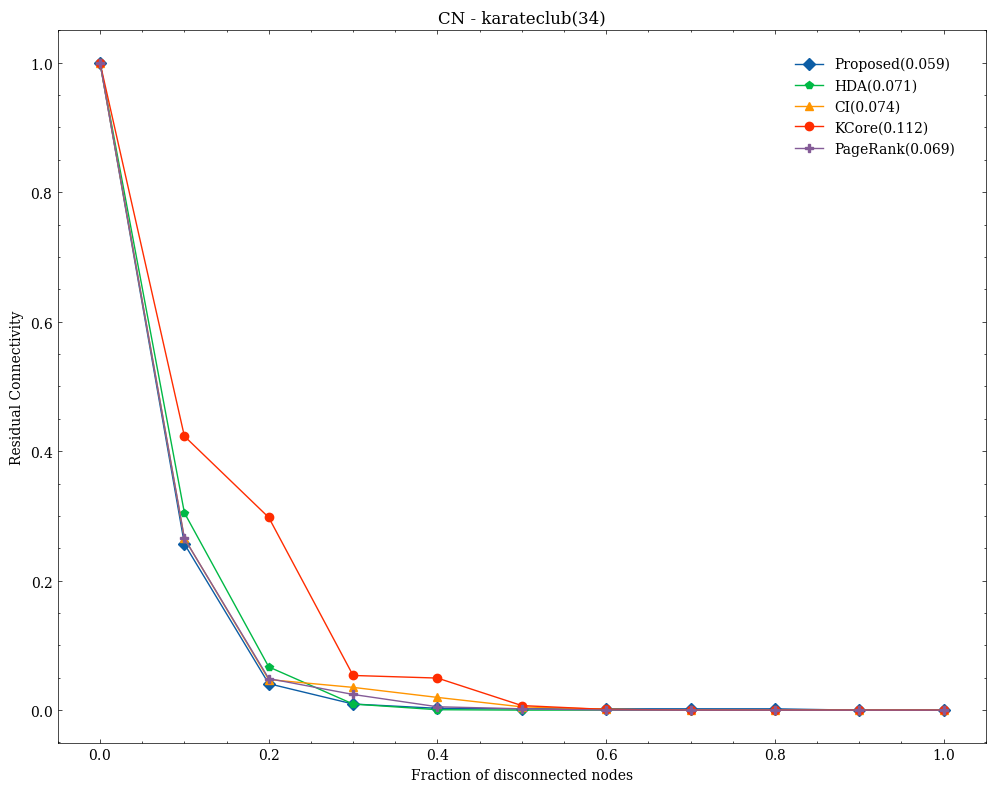
\includegraphics[width=\linewidth]{ANC_CN_karateclub.png}
%         \caption{CN - karateclub}
%     \end{subfigure}%
%     \hfill
%     \begin{subfigure}{0.32\textwidth}
%         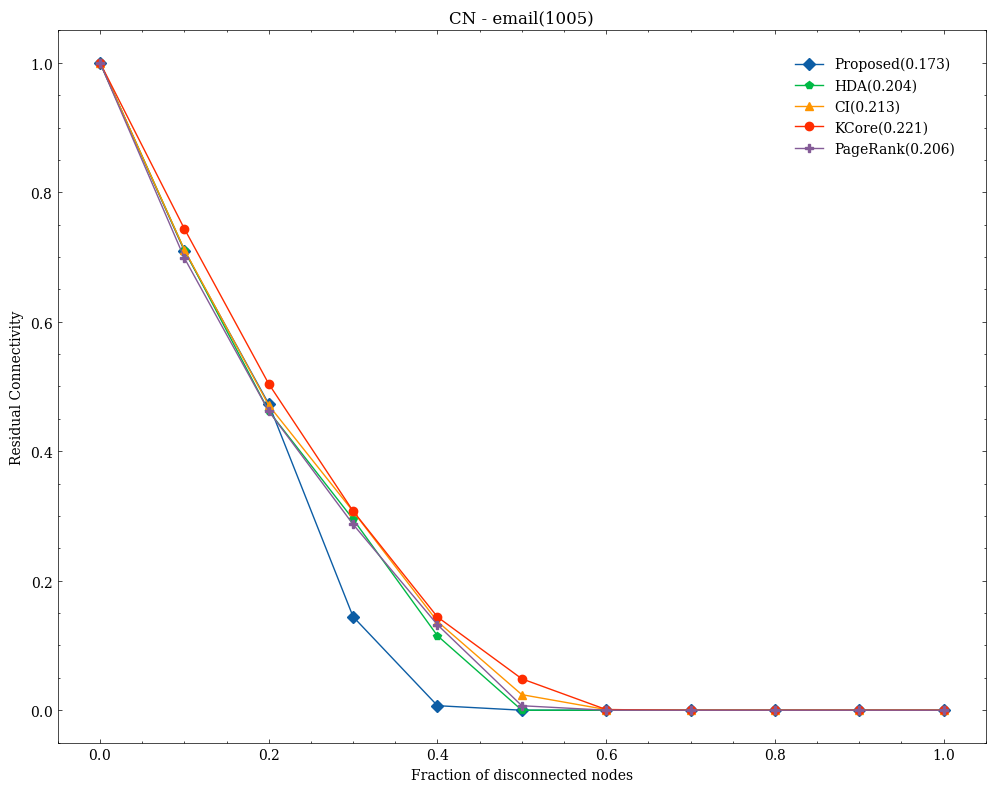
\includegraphics[width=\linewidth]{ANC_CN_email.png}
%         \caption{CN - airport}
%     \end{subfigure}%
%     \hfill
%     \begin{subfigure}{0.32\textwidth}
%         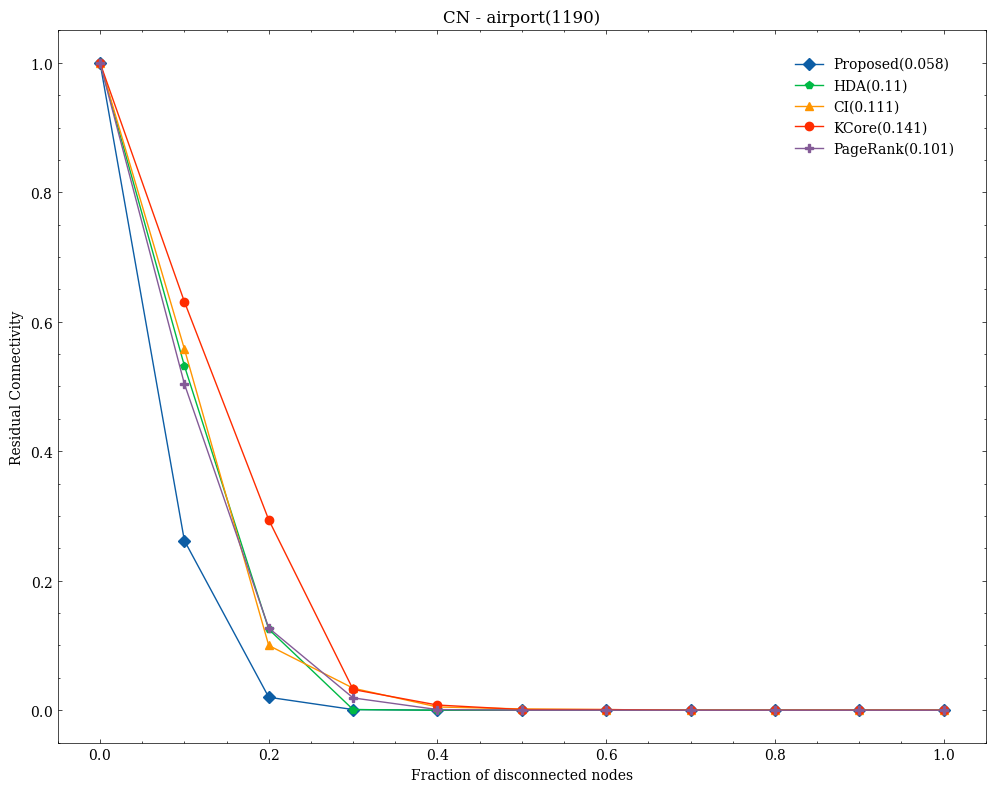
\includegraphics[width=\linewidth]{ANC_CN_airport.png}
%         \caption{CN - airport}
%     \end{subfigure}%

%     \medskip

%     \begin{subfigure}{0.32\textwidth}
%         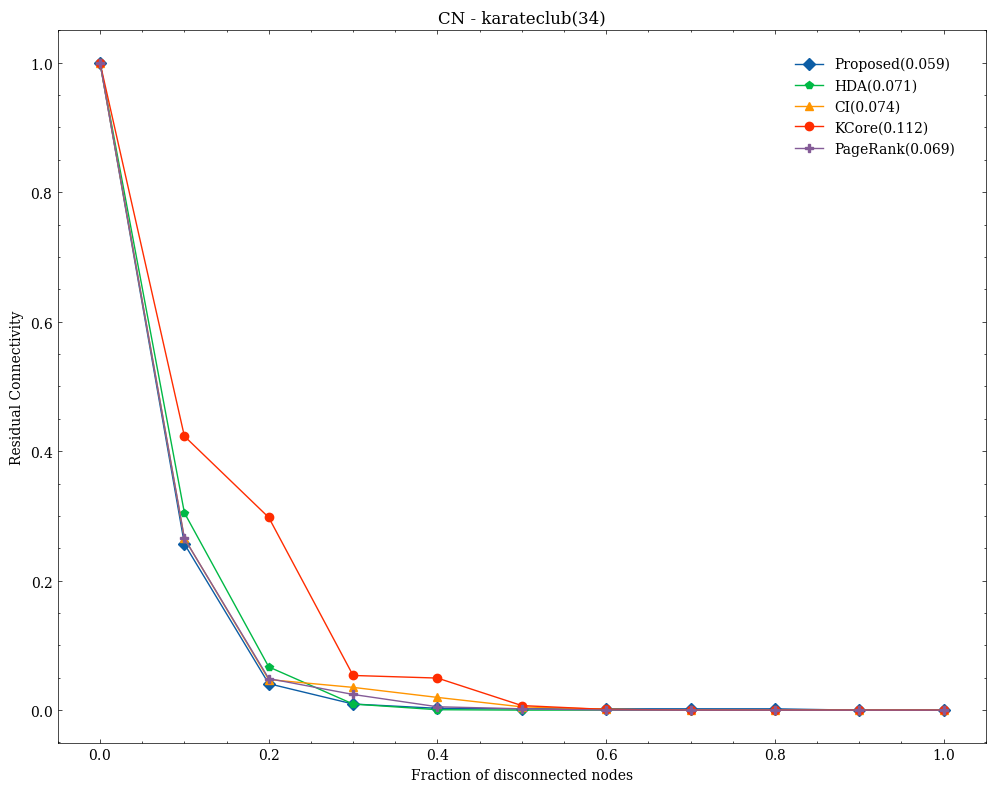
\includegraphics[width=\linewidth]{ANC_CN_karateclub.png}
%         \caption{ND - karateclub}
%     \end{subfigure}%
%     \hfill
%     \begin{subfigure}{0.32\textwidth}
%         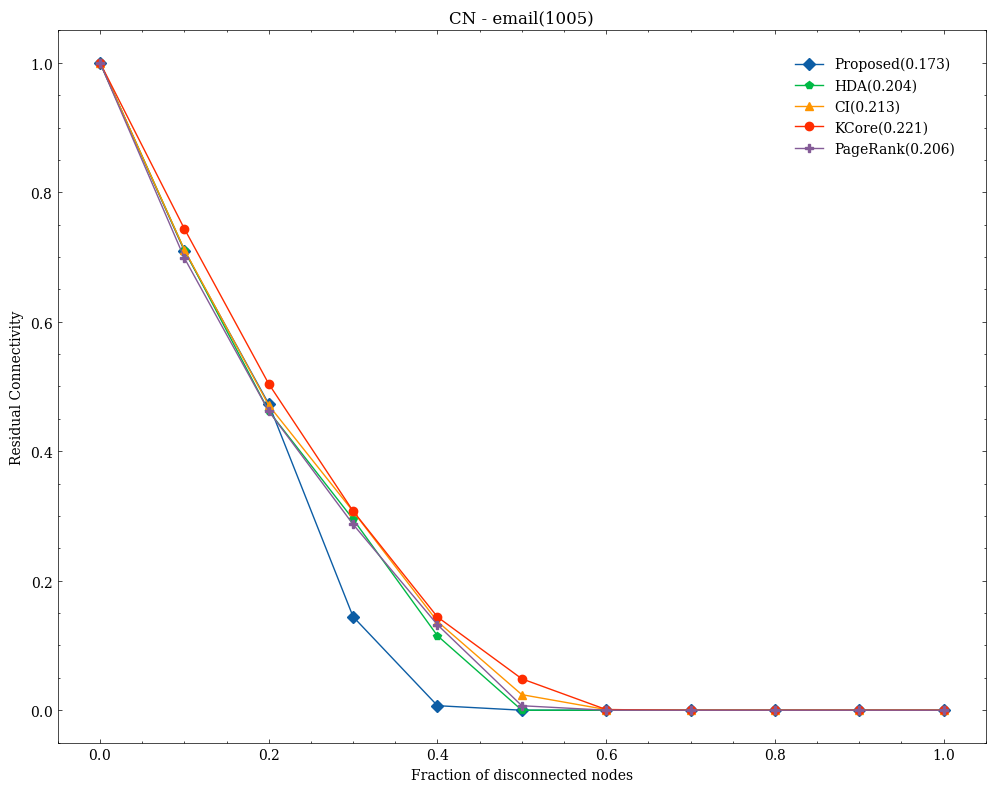
\includegraphics[width=\linewidth]{ANC_CN_email.png}
%         \caption{ND - airport}
%     \end{subfigure}%
%     \hfill
%     \begin{subfigure}{0.32\textwidth}
%         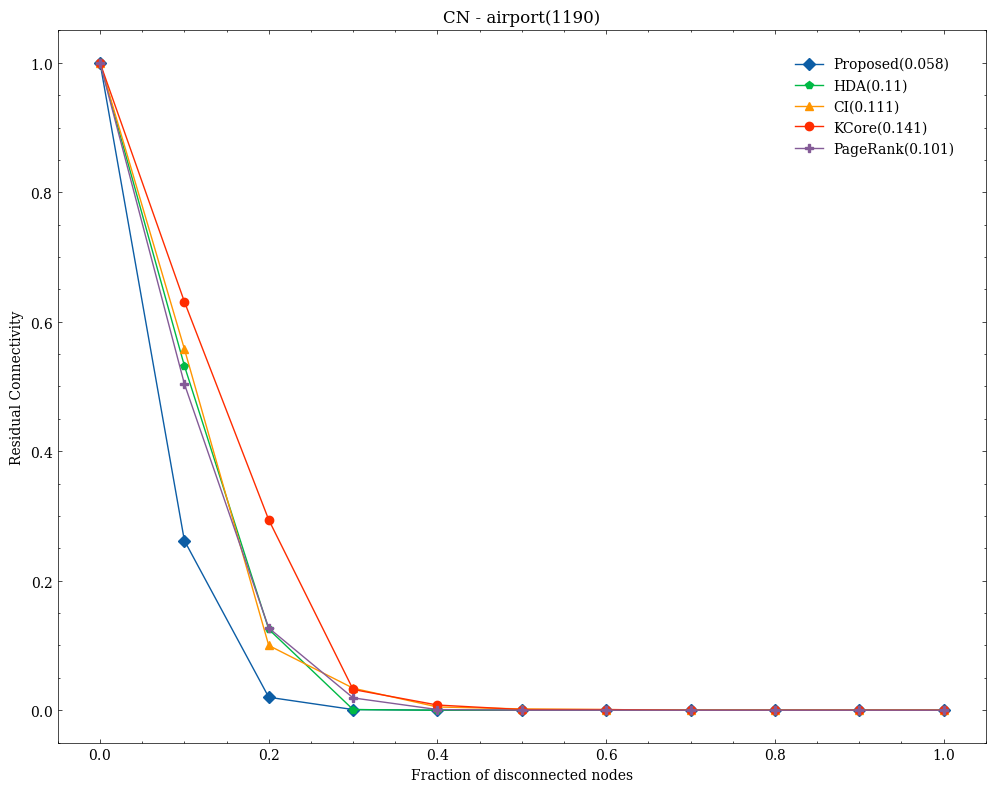
\includegraphics[width=\linewidth]{ANC_CN_airport.png}
%         \caption{ND - airport}
%     \end{subfigure}%
%     \caption{真实数据集上不同算法剩余连接性关于断连节点比例的变化曲线}
%     \label{fig:真实数据集-ANCCurve}
% \end{figure*}

\begin{figure*}[htbp]
    \centering
    \begin{subfigure}{0.45\textwidth}
        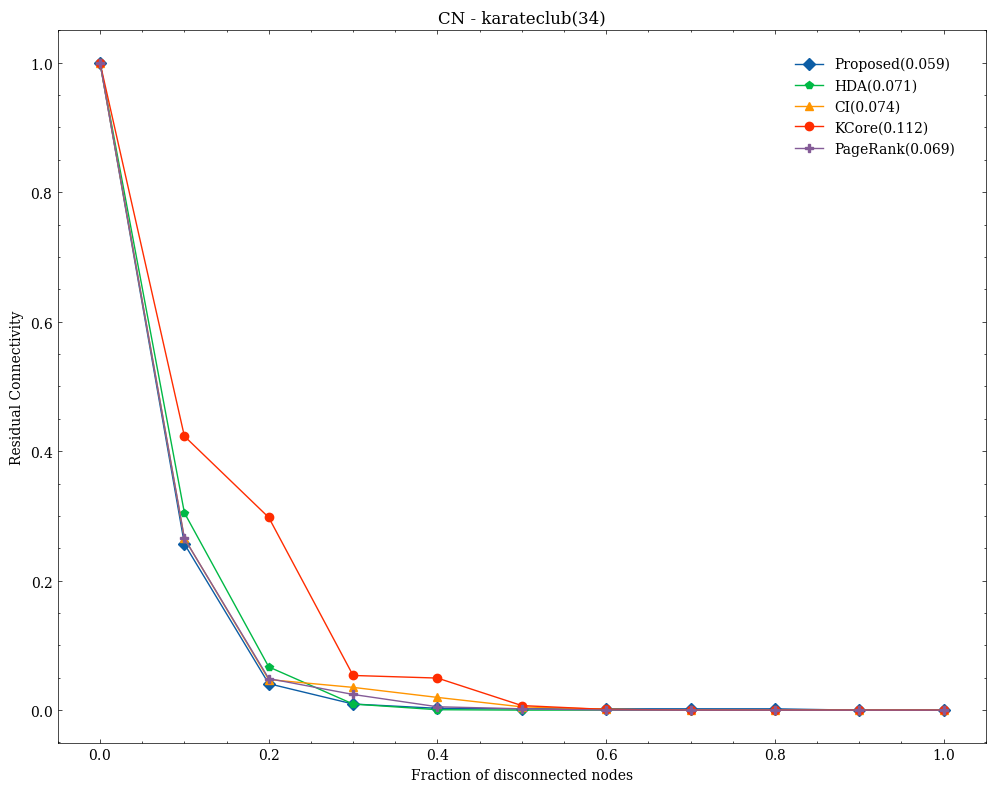
\includegraphics[width=\linewidth]{ANC_CN_karateclub.png}
        \caption{CN - karateclub}
    \end{subfigure}%
    % \hfill
    % \begin{subfigure}{0.24\textwidth}
    %     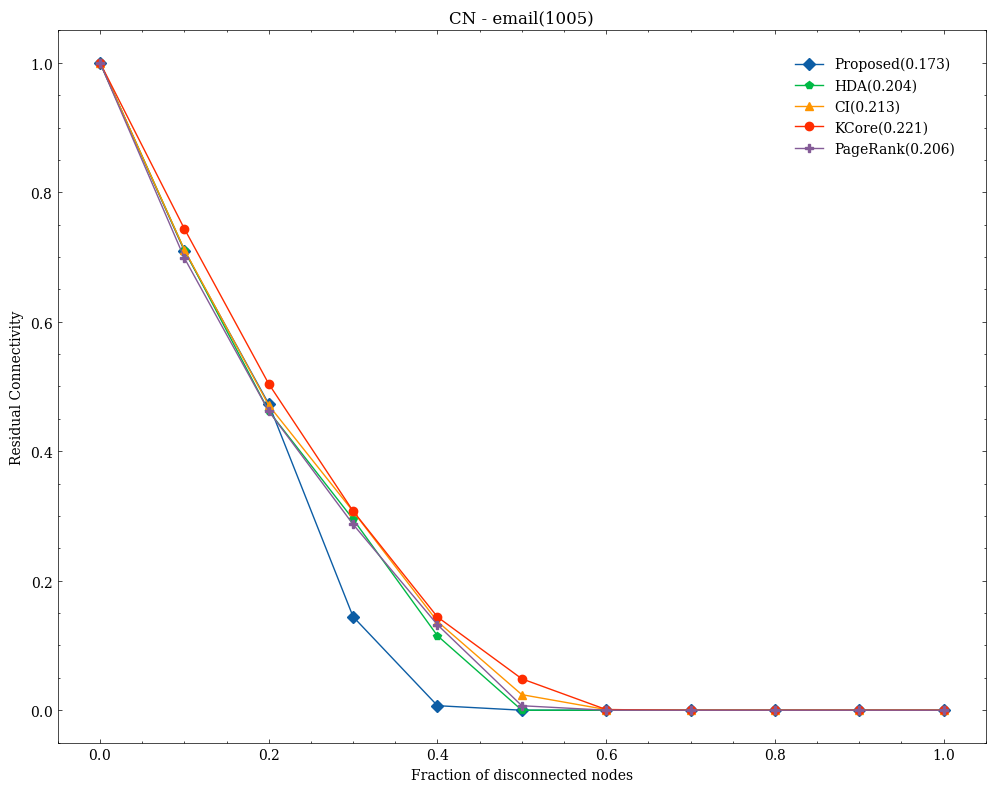
\includegraphics[width=\linewidth]{ANC_CN_email.png}
    %     \caption{CN - airport}
    % \end{subfigure}%
    \hfill
    \begin{subfigure}{0.45\textwidth}
        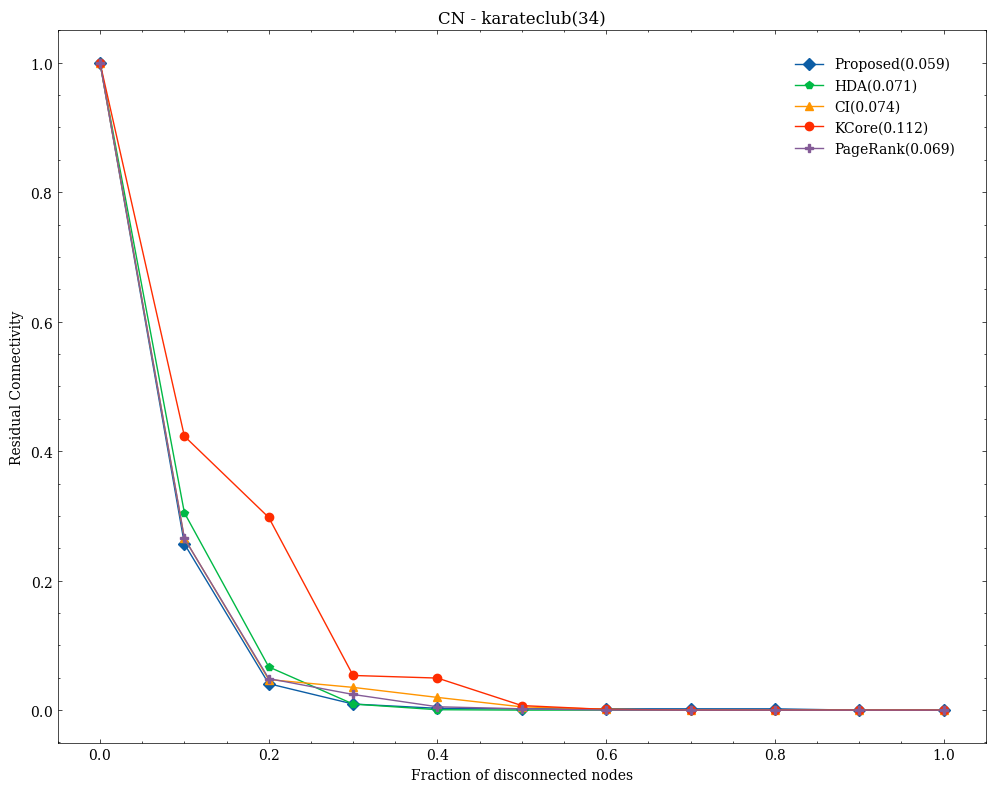
\includegraphics[width=\linewidth]{ANC_CN_karateclub.png}
        \caption{ND - karateclub}
    \end{subfigure}%
    % \hfill
    % \begin{subfigure}{0.24\textwidth}
    %     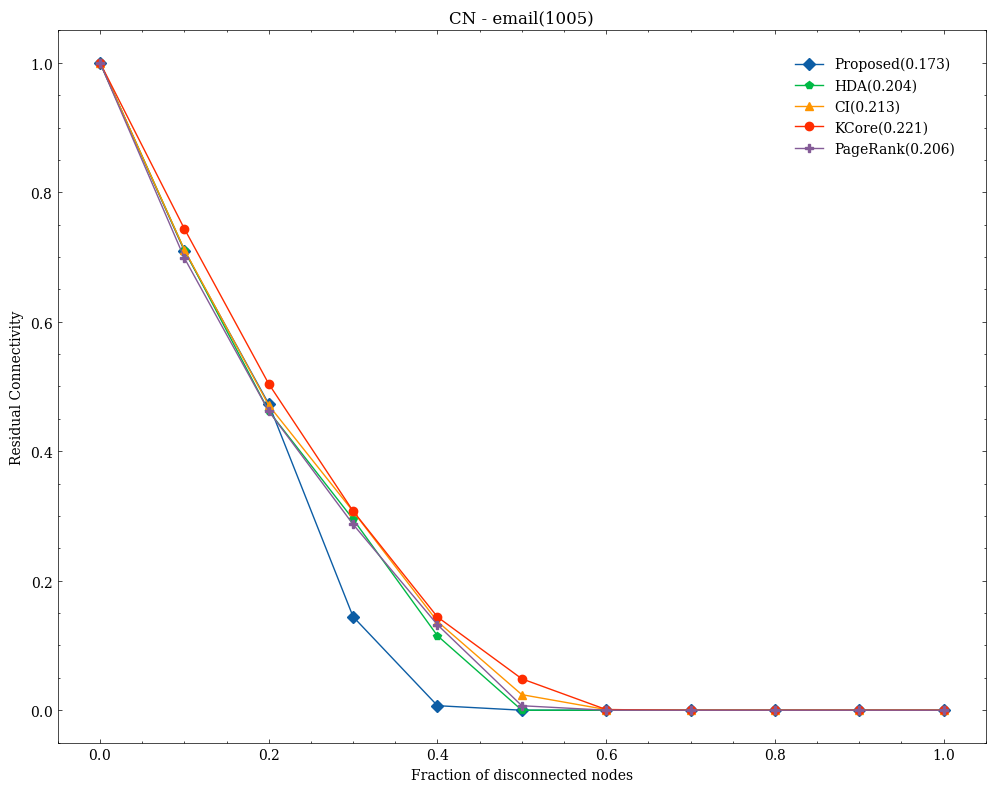
\includegraphics[width=\linewidth]{ANC_CN_email.png}
    %     \caption{ND - airport}
    % \end{subfigure}%
    \caption{真实数据集上不同算法剩余连接性关于断连节点比例的变化曲线}
    \label{fig:真实数据集-ANCCurve}
\end{figure*}
\begin{table*}[hptb]
    \centering
    \begin{tabular}{ccccccccccc}
        \thickhline 
        Algorithm   & \multicolumn{2}{c}{Proposed} & \multicolumn{2}{c}{HDA} & \multicolumn{2}{c}{CI} & \multicolumn{2}{c}{K-Core} & \multicolumn{2}{c}{PageRank} \\
        ProblemType &      CN      &      ND       &     CN     &     ND     &     CN     &    ND     &     CN      &      ND      &      CN      &      ND       \\
        \hline
        karateclub  &     0.059    &     0.135     &    0.071   &    0.137   &   0.074    &   0.153   &    0.112    &     0.225    &     0.069    &     0.138     \\
        email       &     0.173    &     0.232     &    0.204   &    0.287   &   0.213    &   0.314   &    0.221    &     0.323    &     0.206    &     0.301     \\
        bible       &     0.075    &     0.099     &    0.100   &    0.132   &   0.110    &   0.163   &    0.124    &     0.187    &     0.098    &     0.135     \\
        airport     &     0.058    &     0.097     &    0.110   &    0.157   &   0.111    &   0.176   &    0.141    &     0.207    &     0.101    &     0.160     \\
        euroroad    &     0.015    &     0.023     &    0.046   &    0.066   &   0.055    &   0.092   &    0.160    &     0.242    &     0.049    &     0.072     \\
        beacxc      &     0.286    &     0.400     &    0.303   &    0.430   &   0.332    &   0.499   &    0.316    &     0.470    &     0.316    &     0.467     \\
        diseasome   &     0.011    &     0.024     &    0.022   &    0.035   &   0.057    &   0.098   &    0.108    &     0.168    &     0.019    &     0.035     \\
        \thickhline
        \end{tabular}
    \caption{真实数据集上不同算法的ANC数值}
    \label{table:真实数据集-ANCTable}
\end{table*}


\subsubsection{复杂度}\label{sec:Complexity}

首先,我们对时间复杂度进行深入分析。
根据第\ref{sec:Accuracy}节的研究结果表明,那些准确度较高的传统算法往往采用了基于状态的贪心策略(Adaptive)。
即,需要根据当前的状态信息确定影响力最大的节点,并在断连该节点后重新计算每个节点影响力,以确定下一状态影响力最大的节点。
因而,这一类类算法的时间复杂度基本都在$O(|V|^3)$以上。
然而,我们所提出的算法在预测时仅需进行$|V|$次神经网络的前向传播,在GPU的条件下,其时间复杂度相当低。

其次,在空间复杂度方面,我们的算法与传统朴素算法相比具有明显优势。
由于我们的算法无需存储每个状态下节点断连的价值,因此其空间复杂度大大低于朴素算法,在当前存储设备可接受的范围内。


\section{总结}\label{sec:Conclusion}

在复杂网络领域,节点影响力评估这一研究方向一直备受关注。
本文首先从网络拆解的角度提出了节点影响力的朴素算法,并分析了其存在的计算复杂度问题。
其次构建了一个深度强化学习模型,旨在确定最优的网络拆解策略,进而有效排序节点的影响力。
最后通过真实网络上的仿真表明,该算法在复杂度和准确度方面均表现优异,且具备良好的泛化能力和实用性。
然而,尽管取得了显著成果,但该算法尚未提供针对特定时变网络的处理机制,未来的研究可以探索针对特定时变网络进行微调的方法,以进一步提高算法的适用性和效果。

\addbib{references.bib}

\end{document}